%!TEX root = ../../../thesis.tex

This chapter demonstrates an energy harvesting device capable of harvesting energy from flowing water with no moving parts.
A `smart' use for such a harvester is discussed in Chapter~\ref{chap:wirelessWaterMetering}.
I find the minimum power a harvester needs to harvest in order to be useful in chapter \ref{chap:energyRequirements}.
And finally, in chapter \ref{chap:part_1_discussion}, I discuss the design of a harvester and comment on its feasibility.

\section{Operational Model}

In this section we will develop a model of operation for a streaming cell.
This helps to determine what parameters are important when maximising the output power of a cell.

\subsection{Mathematics of streaming}

Mathematical analysis of streaming cells provides a basic understanding of the parameters involved with their output and geometry.
Rigorous mathematical analysis of streaming cell performance is extremely involved and is well detailed in the literature~\cite{Yang1998}.
As aspects of a double layer's structure are still not fully understood, the mathematics behind them is still being developed.
Computer simulation and mathematical modelling are shedding light on the way that ions pack themselves at an electrodes surface~\cite{Kornyshev2007}.
Thus, I have not attempted to model a streaming cell in operation, but instead piece together a model that illustrates the basic concept.

\subsubsection*{Streaming voltage}
\Cref{eq:streamingVoltage_with_pressure} relates the streaming voltage of a parallel plate channel to a pressure differential placed across it.
Gu and Li derived this equation as a means of finding the zeta potential at a water/glass interface~\cite{Gu2000a}.


\begin{equation}
\frac{V_{s}}{\Delta P} = \frac{\varepsilon_{r}\,\varepsilon_{0}\,\zeta}{\mu(\lambda_{b}+\frac{2}{\delta}\lambda_{S})}
\label{eq:streamingVoltage_with_pressure}
\end{equation}
\noindent where:
\begin{description}
    \item $V_{s}$ is the streaming voltage
    \item $\Delta P_{z}$ is the pressure differential across the channel
    \item $\epsilon_{r}$ is the relative permittivity of the liquid
    \item $\epsilon_{0}$ is the absolute permittivity of free space
    \item $\zeta$ is the zeta potential of the solid-liquid interface
    \item $\mu$ is the viscosity of the working fluid
    \item $\lambda_{b}$ is the bulk conductivity of the liquid
    \item $\delta$ is the height of the channel
    \item $\lambda_{s}$ is the surface conductivity of the channel
\end{description}
This equation is specific to parallel plate channels, of the type constructed in the following section.
It requires that the width to height ratio of the channel is greater than 20, which for the case of the cells constructed here it is.
Later, we will measure the streaming voltage to applied pressure ratio; which should allow us to determine both the surface conductivity (Stern conductance) and zeta potential of our channels.

\subsubsection*{Streaming current}
From that same paper, \cite{Gu2000}, the streaming current driven through a rectangular streaming cell was found to be equal to
\begin{equation}
    \frac{I_{s}}{\Delta P} = \frac{\varepsilon_{r}\,\varepsilon_{0}\,\zeta\,W\,\delta}{\mu\,L}
    \label{eq:StreamingCell_StreamingCurrentFunc}
\end{equation}
where
\begin{description}
    \item $W$ is the width of the channel
    \item $L$ is the length of the channel
\end{description}
This equation is similar to that given by Olthuis et al.\ for a porous plug, but has been derived specifically for rectangular channels\cite{Olthuis2005}.

% To help model the situation it is convenient to break \cref{eq:StreamingCell_StreamingCurrentFunc} down in the following
% manner:

% \pagebreak
% \begin{align}
%     I_{s} & = \Delta P\,\left(\frac{A}{\eta\,l}\right)\,\left(\varepsilon_{0}\,\varepsilon_{r}\,\zeta\right)\nonumber\\
%     \label{eq:streaming_current_rearranged}I_{s} & = \frac{\Delta P}{\left(\frac{\eta\,l}{A}\right)}\,\left(\varepsilon_{0}\,\varepsilon_{r}\,\zeta\right)
% \end{align}

% This is a useful step since $\frac{\eta\,l}{A}$ is equivalent to the hydrostatic resistance of the channel.
% Knowing this, we can substitute this hydrostatic resistance into \cref{eq:streaming_current_rearranged} as $R_{h}$ and rearrange, yielding

% \begin{align}
%     I_{s} & = \frac{\Delta P}{R_{h}}\,\left(\varepsilon_{0}\,\varepsilon_{r}\,\zeta\right)\nonumber\\
%     \frac{I_{s}}{\Delta P} & =\frac{\varepsilon_{0}\,\varepsilon_{r}\,\zeta}{R_{h}}\nonumber \\
%     g_{m} & = \frac{\varepsilon_{0}\,\varepsilon_{r}\,\zeta}{R_{h}}
% \end{align}

% where $R_{h}$ is the hydrodynamic resistance caused by the channel, $g_{m}$ represents the transconductance between pressure applied and current produced and $I_{s}$ is the streaming current.
% The hydrodynamic resistance ($R_{h}$) will be affected by the geometry of the channel so $R_{h}$ is considered an approximation of the hydrodynamic resistance.

% Once the cell begins to separate charge, a current in the reverse direction is established called the conduction current ($I_{c}$).

% As Ohm's law states:

% \[ I=\frac{V}{R} \]

% In this situation the resistance is determined by the conductivity of the water
% ($\sigma$), as well as the cross sectional area ($A$) and length ($l$) of the
% channel.

% \[ R=\frac{l}{\sigma\, A} \]


% Therefore, the conduction current back through the channel is determined by:

% \begin{equation} I_{c}=A\sigma\frac{V_{s}}{l} \end{equation}


% Where $\sigma$ is the conductivity of the liquid and $V_{s}$ is the voltage
% developed across the channel.

% At equilibrium the streaming current ($I_{s}$) and the conduction current
% ($I_{c}$) are equal and opposite in direction.


\subsection{\label{sub:Electrical-model}Electrical model}

Figure \ref{fig:StreamingCell_Schematic-representation} depicts schematically how a streaming cell would operate when connected to an external load.
A model of this sort is commonly used to analyse the behaviour transistors.

The model shown here is based upon that found in the work of Olthuis et al.\ in \cite{Olthuis2005}, but has been modified slightly.
Instead of showing $\zeta$ as the equivalent voltage source, it is shown here instead with the pressure applied ($\Delta P$).
As we have no control of the zeta potential in our application, we will consider it a constant.
However, we will have control of the applied pressure across the cell, which we know is directly proportional to the output voltage.

\begin{figure}
    \centering
        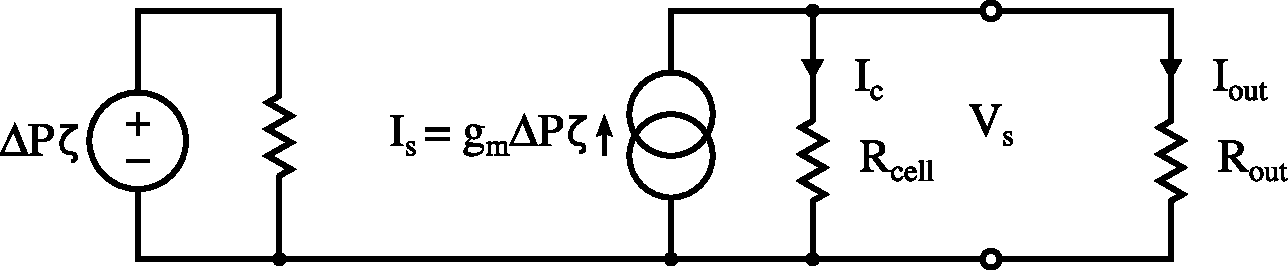
\includegraphics[width=\textwidth]{content/pt1/01-PowerHarvesting/graphics/StreamingCell_EquivalentCircuit_output}
    \caption{\label{fig:StreamingCell_Schematic-representation}Schematic representation, commonly used in electronics, of a streaming cell with attached output resistance}
\end{figure}
In this model the parameter $g_{m}$ is taken from \cref{eq:StreamingCell_StreamingCurrentFunc} as:
\begin{equation}
    g_{m} = \frac{\varepsilon_{r}\,\varepsilon_{0}\,\zeta\,W\,\delta}{\mu\,L}
\end{equation}

The model aids analysis in that it shows the electrical configuration of an external load resistance ($R_{out}$).
We will now determine how this affects the output of the cell and determine how best to extract energy from the cell.

\subsection{Output analysis}

The model thus far contains the parameters necessary to optimise the power output.
We just saw that by placing a load across the cell we are in-fact placing it in parallel with the cell's internal electrical resistance.
In such situations it becomes important to select values of resistance to optimise the cell for either maximum efficiency or maximum power.
So which do we wish to optimise for?

Streaming cells are not batteries.
The only time we can extract energy from a streaming cell is when pressure developed across it, which in tern is because of liquid flowing through it.
When harvestable power is available, we need to collect as much of it as possible -- \emph{no matter how much is wasted}.
Because a cell is incapable of storing energy, any energy that we could not capture will be lost.

The story is different for battery applications.
In those situations it may, but not necessarily, be advantageous to optimise for maximum efficiency.
Doing so will conserve the energy in a battery and ensure that as little as possible goes to waste.
This might be something a cell phone designer aims to achieve, but less important for batteries accelerating an electric car.

In situations requiring maximum efficiency, the efficiency of the system approaches \SI{100}{\percent} as the power delivered approaches \SI{0}{\percent}.
In situations requiring maximum power, the maximum achievable efficiency is \SI{50}{\percent}.
This means we can only harness half of the electrical power developed by a cell, at best.

\subsubsection*{Optimising $R_{out}$ for maximum power}

Using Ohm's Law it is possible to form an equation linking the total power ($P_{cell}$) to the total electrical resistance across the cell ($R_{tot}$).

\begin{eqnarray}
    P & = & V\times I\nonumber \\
    V & = & I\times R\nonumber \\
    P & = & I^{2}\times R\nonumber \\
    P_{cell} & = & I_{s}^{2}\times R_{tot}
    \label{eq:DeterminingOutputPower_basic}
\end{eqnarray}

Where $I_{s}$ is the streaming current created by pumping ions through the channel.
As the output resistance and internal cell resistance are in parallel we can find the output current ($I_{out}$) by treating the cell as a resistor divider (as is shown in~\cref{fig:StreamingCell_Schematic-representation}).
Using a risistor divider equation for current in parallel branches yields:
\begin{eqnarray}
    I_{out} & = & I_{s}\times\frac{R_{cell}}{R_{cell}+R_{out}}
    \label{eq:DeterminingOutputPower_extended}
\end{eqnarray}

Combining \eqref{eq:DeterminingOutputPower_basic} and \eqref{eq:DeterminingOutputPower_extended} we can extract the power dissipated in a load attached across the cell.

\begin{eqnarray}
    I_{out} & = & I_{s}\times\frac{R_{cell}}{R_{cell}+R_{out}}\nonumber \\
    P_{out} & = & \left[I_{s}\times\frac{R_{cell}}{R_{cell}+R_{out}}\right]^{2}\times R_{out}
    \label{eq:DeterminingOutputPower_result}
\end{eqnarray}

Equation \eqref{eq:DeterminingOutputPower_result} takes into account the internal dissipation within the cell due to its own internal resistance.
In order to optimise the output power it is necessary to find the value of output resistance ($R_{out}$) that maximises the output power.

A parallel resistance system where we try to maximise the output power suggests this is a maximum power transfer theorem problem.
The maximum power transfer theorem states that in order to maximise the power delivered to an external load from a source which itself has an internal resistance, one must make the two resistance equal.

\subsubsection*{Maximum power transfer theorem for a current source}
This theorem is shown for resistors in series but no clear proof was found for a current source with two resistances in parallel.
Here I prove that the maximum power theorem holds for a current source with resistors in parallel.
This is not new work, but is included for completeness.

First we take \cref{eq:DeterminingOutputPower_result} and treat the streaming current ($I_{s}$) as a constant, differentiate with respect to $R_{out}$ and find the condition that gives a maximum/minimum power output.
\begin{eqnarray}
    P_{out} & = & \left[I_{s}\times\frac{R_{cell}}{R_{cell}+R_{out}}\right]^{2}\times R_{out}\nonumber\\
    \frac{P_{out}}{R_{out}} & = & \left[1\times\frac{R_{cell}}{R_{cell}+R_{out}}\right]^{2}\nonumber\\
    \frac{\partial P_{out}}{\partial R_{out}} & = & \frac{R_{cell}^{2}}{(R_{cell}+R_{out})^{2}}-\frac{2\times R_{cell}^{2}\times R_{out}}{(R_{cell}+R_{out})^{3}}\nonumber\\
    0 & = & \frac{R_{cell}^{2}}{(R_{cell}+R_{out})^{2}}-\frac{2\times R_{cell}^{2}\times R_{out}}{(R_{cell}+R_{out})^{3}}\nonumber\\
    \frac{2\times R_{cell}^{2}\times R_{out}}{(R_{cell}+R_{out})^{3}} & = & \frac{R_{cell}^{2}}{(R_{cell}+R_{out})^{2}}\nonumber\\
    \frac{2\times R_{cell}^{2}\times R_{out}}{R_{cell}+R_{out}} & = & R_{cell}^{2}\nonumber\\
    2\times R_{cell}^{2}\times R_{out} & = & R_{cell}^{2}\times(R_{cell}+R_{out})\nonumber\\
    2\times R_{out} & = & R_{cell}+R_{out}\nonumber\\
    R_{out} & = & R_{cell}
    \label{eq:maximumPowerTheorem_norton}
\end{eqnarray}

This shows that there is either maximum or minimum power transfer to $R_{out}$ when the value of $R_{out}$ matches that of $R_{cell}$.
By plotting the power output as a function of the ratio of the two resistances (shown in \cref{fig:Plot-of-PowerTheorem}), we can see it is indeed a maximum.
This shows the assumption of the maximum power transfer theorem in the case of streaming cell output to be correct.
Usefully, it is shown that the absolute magnitudes of both $R_{out}$ and $R_{cell}$ have no effect on the output power - only their relative sizes (which in this case is equal).

\begin{figure}
    \centering
        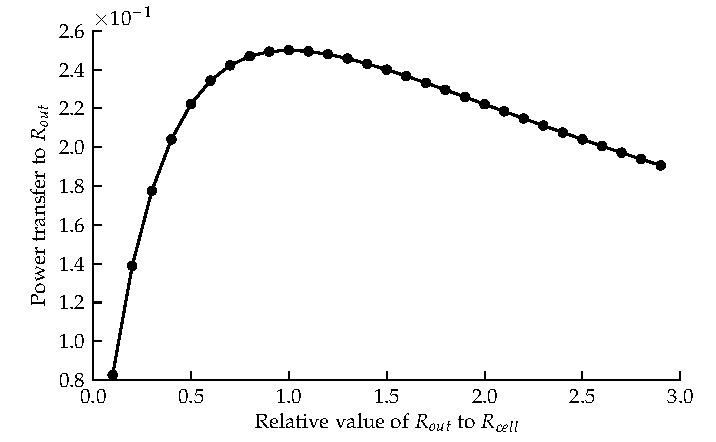
\includegraphics{content/pt1/01-PowerHarvesting/graphics/maximumPowerThereom}
    \caption{\label{fig:Plot-of-PowerTheorem}Plot of Equation \ref{eq:DeterminingOutputPower_result} when $I_{s}=1A$ and $R_{cell}=1\Omega$}
\end{figure}

\subsubsection*{Optimising streaming cell parameters}

We now use the optimised values of $R_{out}$ and $R_{cell}$ to calculate the maximum available power.
This is done by substituting $R_{out}$ and $R_{cell}$ for simply $R$ in \eqref{eq:DeterminingOutputPower_result} as follows.
\begin{eqnarray}
    P_{out} & = & \left[I_{s}\times\frac{R_{cell}}{R_{cell}+R_{out}}\right]^{2}\times R_{out}\nonumber \\
    P_{max} & = & \left[I_{s}\times\frac{1}{2}\right]^{2}\times R\nonumber \\
    P_{max} & = & \frac{I_{s}^{2}R}{2}
    \label{eq:streamingCell_maxPower}
\end{eqnarray}
As $P=I^{2}R$ (via the power equation and Ohm's Law) this indicates at best we can capture half of the available power.

It is now possible to combine the equation for maximum power, \eqref{eq:streamingCell_maxPower}, and that for streaming current, \eqref{eq:StreamingCell_StreamingCurrentFunc}.
\begin{eqnarray}
    P_{max} & = & \frac{I_{s}^{2}R}{2}\nonumber \\
    P_{max} & = & \left(\frac{\varepsilon\,\zeta\,W\,\delta\,\Delta P}{\mu\,L}\right)^{2}\times\frac{R}{2}
    \label{eq:streamingCell_maxPower_substituted}
\end{eqnarray}
where $\varepsilon=\varepsilon_{0}\,\varepsilon_{r}$ and $R=R_{cell}=R_{out}$.

To get a better feel for this equation, it may help to substitute in the parameters that affect $R$.
From here we will refer to $R$ as the internal electrical resistance of the cell.
It also refers to the external resistance in the maximum power condition, but we are free to vary that to match the internal resistance.

We begin with the understanding that:
\begin{eqnarray}
    R & \propto & \frac{L}{A\,\sigma}\label{eq:cell_resistance_electrical}\\
    R_{h} & \propto & \frac{L\,\mu}{A}\label{eq:cell_resistance_hydro}
\end{eqnarray}
where $\sigma$ is the conductivity of the liquid and $A$ is the cross-sectional area of the cell.
The first equation \eqref{eq:cell_resistance_electrical} states that the electrical resistance will increase with cell length and decrease with the cross-sectional area of the cell and the conductivity of the fluid.
The second \eqref{eq:cell_resistance_hydro} states that the fluid mechanical resistance will increase with the length of the cell and the viscosity of the fluid, and decrease with the cross-sectional area of the cell.

We can identify an inverse relationship with hydrostatic resistance in
We can identify the presence of $R_{h}$ in equation \eqref{eq:streamingCell_maxPower_substituted}.
Starting with this equation we substitute equation \eqref{eq:cell_resistance_electrical} in and rearrange to produce an approximate relationship between pressure, cell length and area:
\begin{eqnarray}
    P_{max} & = & \left(\frac{\varepsilon\,\zeta\,W\,\delta\,\Delta P}{\mu\,L}\right)^{2}\times\frac{R}{2}\nonumber\\
    P_{max} & \propto & \left(\frac{W\,\delta}{\mu\,L}\right)^{2}\times\left(\varepsilon\,\zeta\,\Delta P\right)^{2}\times \frac{L}{A\,\sigma} \times\frac{1}{2}\nonumber\\
    P_{max} & \propto & \left(\frac{A}{\mu\,L}\right)^{2}\times\left(\varepsilon\,\zeta\,\Delta P\right)^{2}\times \frac{L}{A\,\sigma} \times\frac{1}{2}\nonumber\\
    P_{max} & \propto & \frac{A^{2}}{L^{2}}\times\left(\frac{\varepsilon\,\zeta\,\Delta P}{\mu}\right)^{2}\times \frac{L}{A} \times\frac{1}{2\,\sigma}\nonumber\\
    P_{max} & \propto & \frac{A}{L}\times\left(\frac{\varepsilon\,\zeta\,\Delta P}{\mu}\right)^{2}\times\frac{1}{2\,\sigma}\nonumber\\
    P_{max} & \propto & \left(\frac{\varepsilon\,\zeta\,\Delta P}{\mu}\right)^{2}\times\frac{A}{2\,L\,\sigma}\nonumber\\
    P_{max} & \propto & \frac{\Delta P^{2}\,A}{L}\times \frac{\varepsilon^{2}\,\zeta^{2}}{2\,\mu^{2}\,\sigma}
    \label{eq:streamingCell_maxPower_relationship}
\end{eqnarray}

This equation \eqref{eq:streamingCell_maxPower_relationship} suggests that a cell with a small length, large area and high pressure is the best candidate for maximising power output.
When using tap water we have no control over the remaining parameters; highlighting the importance of cell geometry and applied pressure.


% \begin{eqnarray} P_{max} & = & \frac{\Delta
%         P^{2}\,\varepsilon^{2}\,\zeta^{2}R}{2R_{h}^{2}}\nonumber \\ P_{max} & =
%     & \frac{\Delta P^{2}\,\varepsilon^{2}\,\zeta^{2}\,\left(\frac{l}{\sigma\,
%                 A}\right)}{2\left(\frac{\eta\, l}{A}\right)_{h}^{2}}\nonumber
%     \\ P_{max} & = & \frac{\Delta P^{2}\,\varepsilon^{2}\,\zeta^{2}\,
%         l}{\sigma\, A}\times\frac{1}{\frac{2\eta^{2}\, l^{2}}{A^{2}}}\nonumber
%     \\ P_{max} & = & \frac{\Delta P^{2}\,\varepsilon^{2}\,\zeta^{2}\, l\,
%         A^{2}}{\sigma\, A\,2\eta^{2}\, l^{2}}\nonumber \\ P_{max} & = &
%     \frac{\Delta P^{2}\,\varepsilon^{2}\,\zeta^{2}\, A}{2\,\sigma\,\eta^{2}\,
%         l}\nonumber \\ P_{max} & \propto & \frac{\Delta P^{2}\,\zeta^{2}\,
%         A}{l}\nonumber \\ P_{max} & \propto & \frac{\Delta
%         P^{2}\,\zeta^{2}}{R_{h}} \end{eqnarray}



% \subsubsection*{Optimisation of $R_{h}$ and $\Delta P$}

% Knowing the optimum value of output resitance leaves only the streaming current
% ($I_{s}$) and it's constituants as optimisation parameters.  Equation
% \ref{eq:StreamingCurrent_HydrostaticResistance} indicates that in order to
% further optimise the cell, one must reduce hydrodynamic resistance ($R_{h}$)
% and increase both the Zeta potential ($\xi$) and pressure difference ($\Delta
% P$) placed across the cell.

% We can model the water supply, harvester and a consumer as a basic electrical
% circuit as shown in Figure \ref{fig:Schematic-model-of-harvester}.  In this
% model $P_{supply}$ represents the total water pressure available, Flow
% represents the flow rate of water, $R_{h}$ and $R_{consumer}$ are the
% hydrodynamic resistances of the harvesting cell and a water consumer (e.g. a
% house) respecively and $\Delta P$ is the pressure developed difference across
% the harvester, where $R_{h}\propto\frac{l}{A}$.

% \begin{figure} \begin{centering}
%         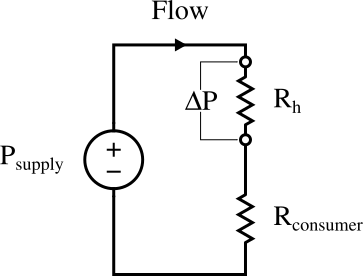
\includegraphics[scale=0.55]{content/pt1/01-PowerHarvesting/graphics/Harvester_equivalentCircuit_output}
%         \par\end{centering}

% \protect\caption{\label{fig:Schematic-model-of-harvester}Schematic model of the
%     water supply, harvester and consumer}


% \end{figure}


% \begin{figure} \begin{centering}
%         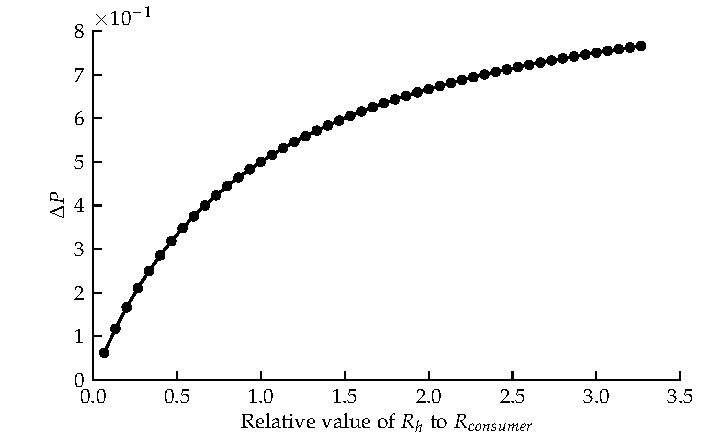
\includegraphics{content/pt1/01-PowerHarvesting/graphics/streamingCell_consumerModel_dP}
%         \par\end{centering}

% \protect\caption{\label{fig:Effect-of-varying-Rh-onP}Effect of varying $R_{h}$
%     on $\Delta P$ for the harvester/consumer model shown in Figure
%     \ref{fig:Schematic-model-of-harvester}.}


% \end{figure}


% \begin{figure} \begin{centering}
%         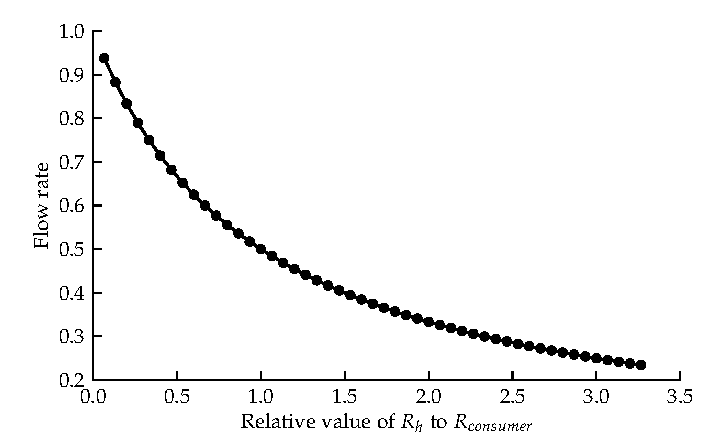
\includegraphics{content/pt1/01-PowerHarvesting/graphics/streamingCell_consumerModel_flow}
%         \par\end{centering}

% \protect\caption{\label{fig:Effect-of-varying-Rh-onFlow}Effect of varying
%     $R_{h}$ on Flow for the harvester/consumer model shown in Figure
%     \ref{fig:Schematic-model-of-harvester}.} \end{figure}


% \begin{figure} \begin{centering}
%         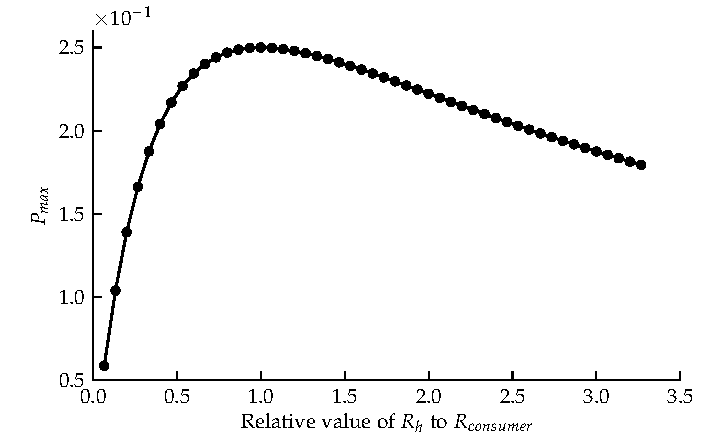
\includegraphics{content/pt1/01-PowerHarvesting/graphics/streamingCell_consumerModel_total}
%         \par\end{centering}

% \protect\caption{\label{fig:Effect-of-varying-Rh-onIs}Effect of varying $R_{h}$
%     on \foreignlanguage{english}{$P_{max}$} for the harvester/consumer model
%     shown in Figure \ref{fig:Schematic-model-of-harvester}.} \end{figure}
% Figures \ref{fig:Effect-of-varying-Rh-onP},
% \ref{fig:Effect-of-varying-Rh-onFlow} and \ref{fig:Effect-of-varying-Rh-onIs}
% show how varying $R_{h}$ will affect $\Delta P$, the flow rate and the value of
% $\frac{\Delta P}{R_{h}}$ respectively. Notice in Figure
% \ref{fig:Effect-of-varying-Rh-onP} that increasing $R_{h}$ has the effect of
% increasing $\Delta P$.  Optimisation wise, the benifit of increasing $I_{s}$ by
% increasing $\Delta P$ is opposed by also increasing the value of $R_{h}$
% (referring to Equation \ref{eq:StreamingCurrent_HydrostaticResistance}).

% Figure \ref{fig:Effect-of-varying-Rh-onFlow} shows how the value of $R_{h}$
% affects the flow rate through the system. Keeping the flow rate high is
% important in order to ensure that the consumer does not notice a drop in water
% pressure due to the addition of the harvester in their water system.

% Finally, Figure \ref{fig:Effect-of-varying-Rh-onIs} shows the effect that
% varying $R_{h}$ has on \foreignlanguage{english}{$P_{max}$} (according to
% $P_{max}\propto\frac{\Delta P^{2}\,\zeta^{2}}{R_{h}}$ when $\zeta=1$). The
% result is the same as that of Equation \ref{eq:DeterminingOutputPower}, showing
% that this is again goverend by the maximum power transfer thereom. Practically,
% a harvester that dropped half of the supply pressure would not be feasable in
% most domestic situations, so a trade-off will have to be made that meets
% plumbing standards.


% \subsubsection*{Optimisation of the Zeta potential}

% Referring back to Equation \ref{eq:StreamingCell_StreamingCurrentFunc}, I have
% determined how to increase the total output of the harvester by choosing
% appropriate values for all of the parameters except $\varepsilon_{r}$ and
% $\zeta$. As the harvester will be using domestic tap water the value of
% $\varepsilon_{r}$ will be that of the relative permittivity of water, and is
% therefore relatively fixed (being only affected by the temperature of the
% water). This leaves $\zeta$ as the remaining parameter.

\section{Building a Streaming Cell}

  Building a streaming cell seemed a simple task at the outset.
  This section gives a brief overview of the work related to creating that first working streaming cell.

  \subsection{First streaming cells}

    \begin{figure}
      \centering
      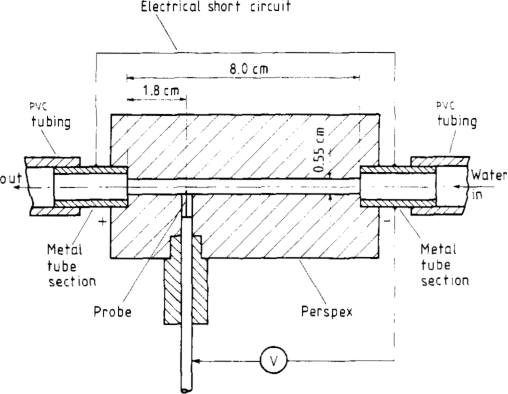
\includegraphics{content/pt1/01-PowerHarvesting/graphics/VargaSeymour1986_cell}
      \caption{\label{fig:first_cell_diagram}Diagram of a cavitation device, taken from ~\cite{Varga1986}, reported to be able to generate over \SI{50}{\volt} across its ends by pumping water through it.}
    \end{figure}

    \begin{figure}
      \centering
      \includegraphics[scale=0.9]{content/pt1/01-PowerHarvesting/graphics/StreamingCell_v0}
      \caption{\label{fig:first_cell}Photo of the first generation of streaming device built, by summer research student Jonathon McMullan, to create the streaming voltages reported by Varga and Seymour.}
    \end{figure}
    \begin{figure}
      \centering
      \includegraphics[scale=0.7]{content/pt1/01-PowerHarvesting/graphics/StreamingCells_v1}
      \caption{\label{fig:first_cells}Photo showing two examples of a second design of streaming cell made entirely from glass.}
    \end{figure}

    The work that first sparked the interest of both my primary supervisor and I in streaming devices was that of Varga and Seymour~\cite{Varga1986}.
    In that paper it was reported that a device employing cavitation as a means of increasing the resistance between two bodies of  water was capable of developing over \SI{50}{\volt} across its ends.
    A diagram of the cavitation device is shown as \cref{fig:first_cell_diagram}.
    An attempt to replicate the results of that paper was made by summer research student Jonathon McMullan.
    Jonathon built a replica of the device, shown as \cref{fig:first_cell}; but was unable to reproduce streaming phenomena.

    My supervisor and I became sceptical of streaming cells at this point and looked elsewhere for energy harvesting ideas.
    The following year, summer research student Wane Crump and I conducted experiments to determine the amount of charge that could be transported on water droplets.
    This work was related to the idea of an electrostatic generator.
    See \cref{appendix:chargedDropletts} for details of the droplet based harvesting research.

    Later, after trawling through the engineering literature I found reports of other designs of streaming cells, namely that of Gu and Li~\cite{Gu2000}.
    Their work convinced me to replicate their design of streaming cells as they appeared relatively simple to fabricate.
    Employing Waikato University's on-site glassblower, Steve Newcombe, two streaming cells were fabricated entirely from soda-lime glass,
    These streaming cells are shown in \cref{fig:first_cells}.

    Each of the two channels were made by placing a \SI{50}{\micro\meter} sheet of copper between the glass slides; then wielding the glass slides together to seal the cell; and finally, etching the copper out with acid.
    The cells were then wielded (with glass) to the two side tubes that held the copper electrodes.
    By varying the length of the two channels (one of \SI{2}{\centi\meter}, the other \SI{4}{\centi\meter}) we hoped to determine what role length played on channel output characteristics.
    Unfortunately, these streaming cells where unable to contain the pressure applied from our lab tap, bursting at or around the glass wields containing the high-pressure water.
    A crack along the right hand reservoir is visible on the \SI{2}{\centi\meter} wide channel.
    Attempts were made to strengthen the channels by coating joins with industrial glues, but none were successful.

 \subsection{Robust streaming cells}

    After the previous attempts to create streaming cells failed, a new, more robust design was employed.
    This design favoured the used of epoxy resin and acrylic to contain the channels.
    Both of these materials allow for more flex without cracking or breaking.
    Much of this design was taken from Gu and Li's paper on zeta potentials of glass and aqueous solutions~\cite{Gu2000}.

    \begin{figure}[p]
      \centering
      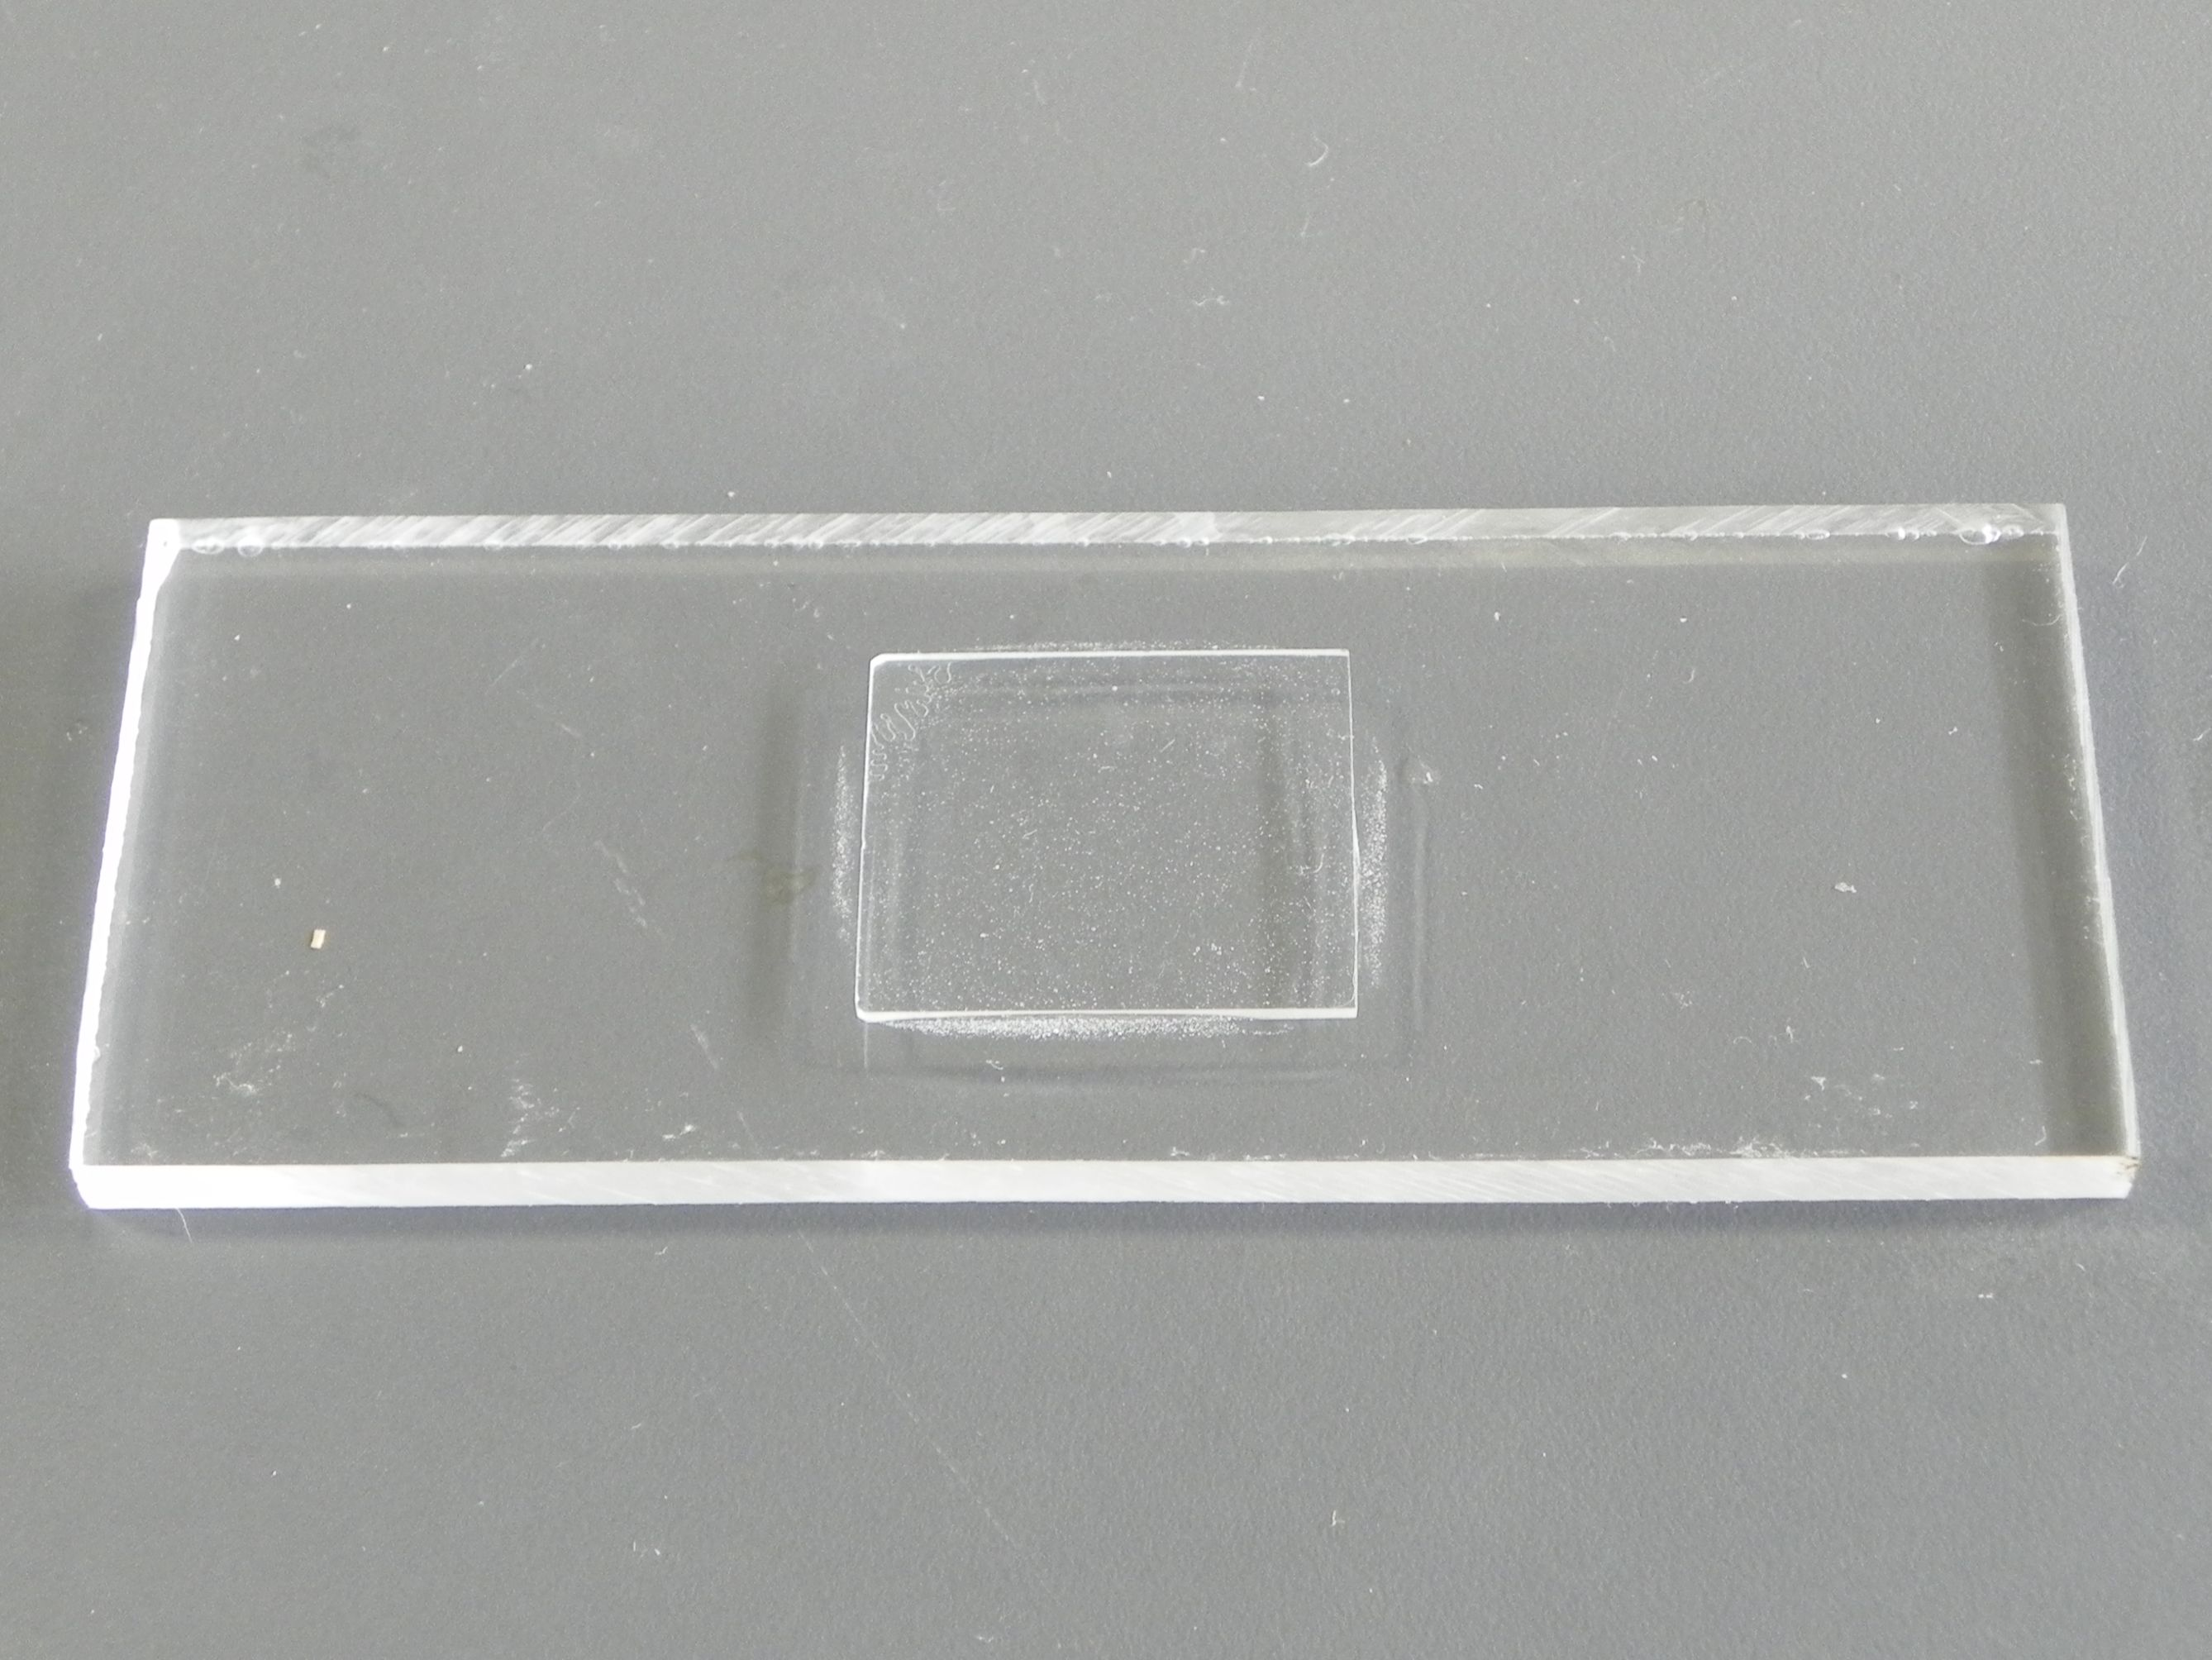
\includegraphics[width=0.5\textwidth]{content/pt1/01-PowerHarvesting/graphics/Photo_streamingPotential_Assembly_Step1.JPG}
      \caption{\label{fig:Photo_streamingPotential_Assembly_Step1}Photo showing half of a glass slide glued to acrylic base plate}
    \end{figure}
    \begin{figure}[p]
      \centering
      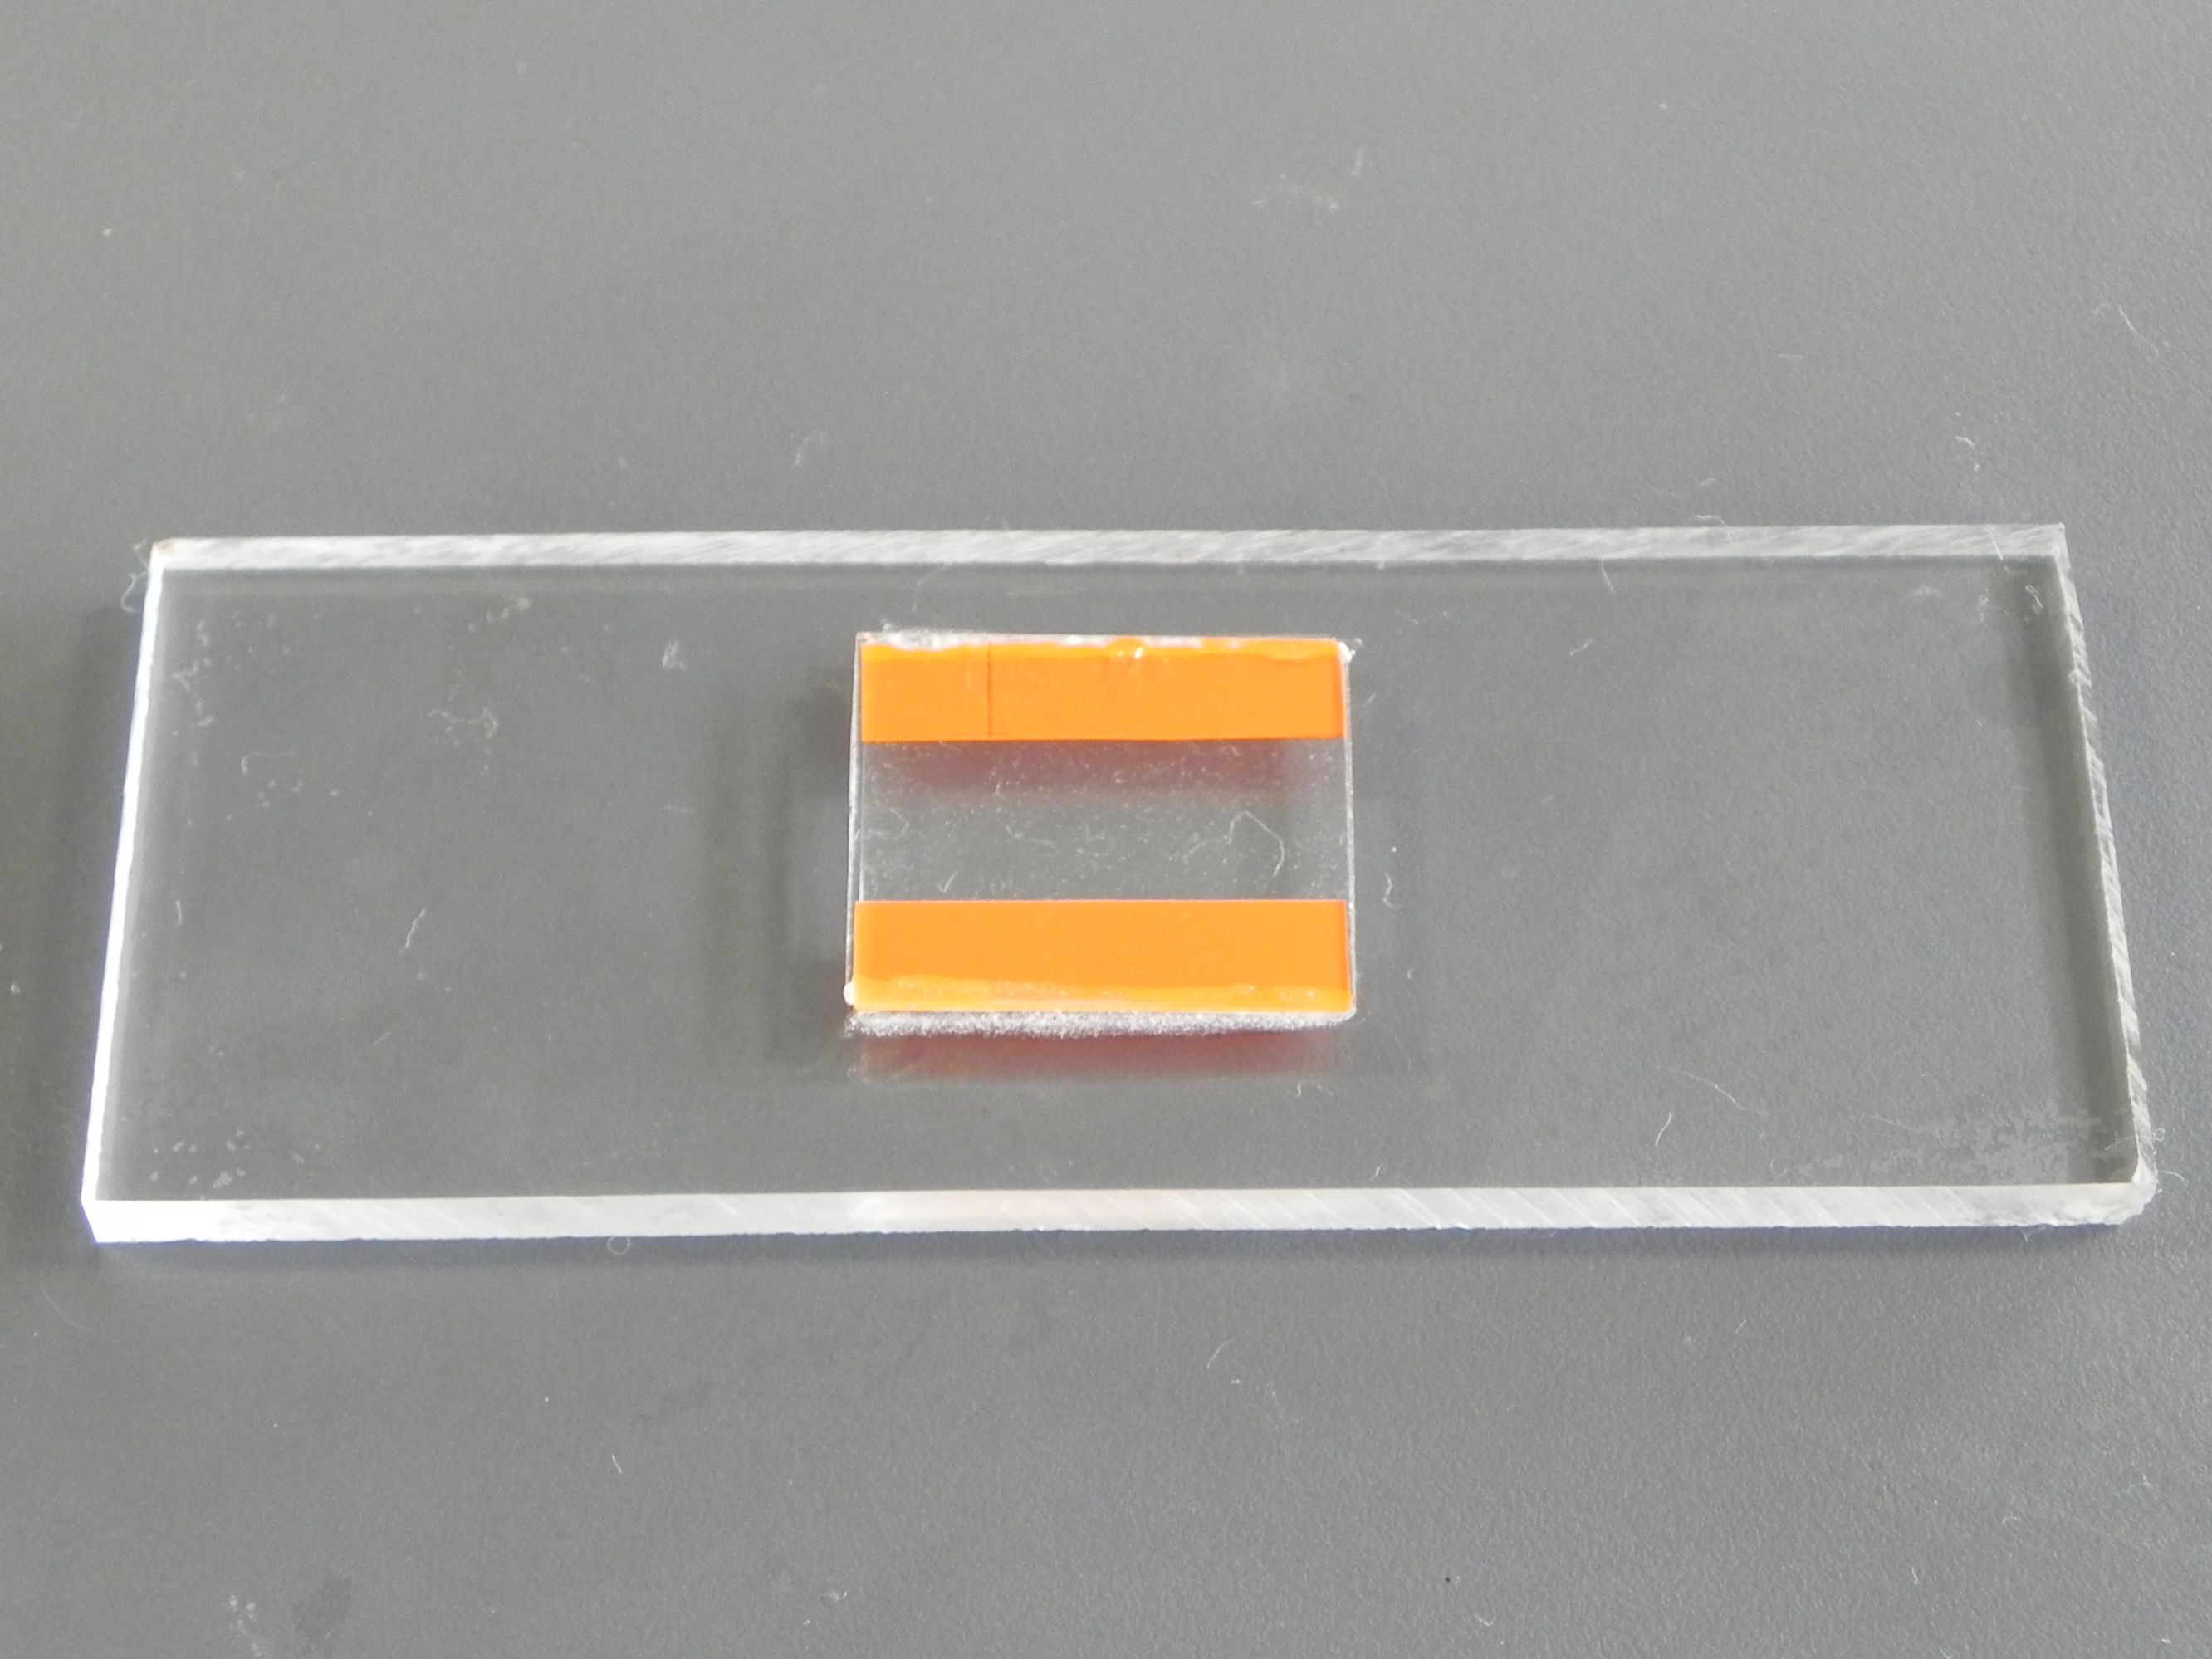
\includegraphics[width=0.5\textwidth]{content/pt1/01-PowerHarvesting/graphics/Photo_streamingPotential_Assembly_Step2.JPG}
      \caption{\label{fig:Photo_streamingPotential_Assembly_Step2}Photo showing plastic shims sandwiched between two slide halves}
    \end{figure}
    \begin{figure}[p]
      \centering
      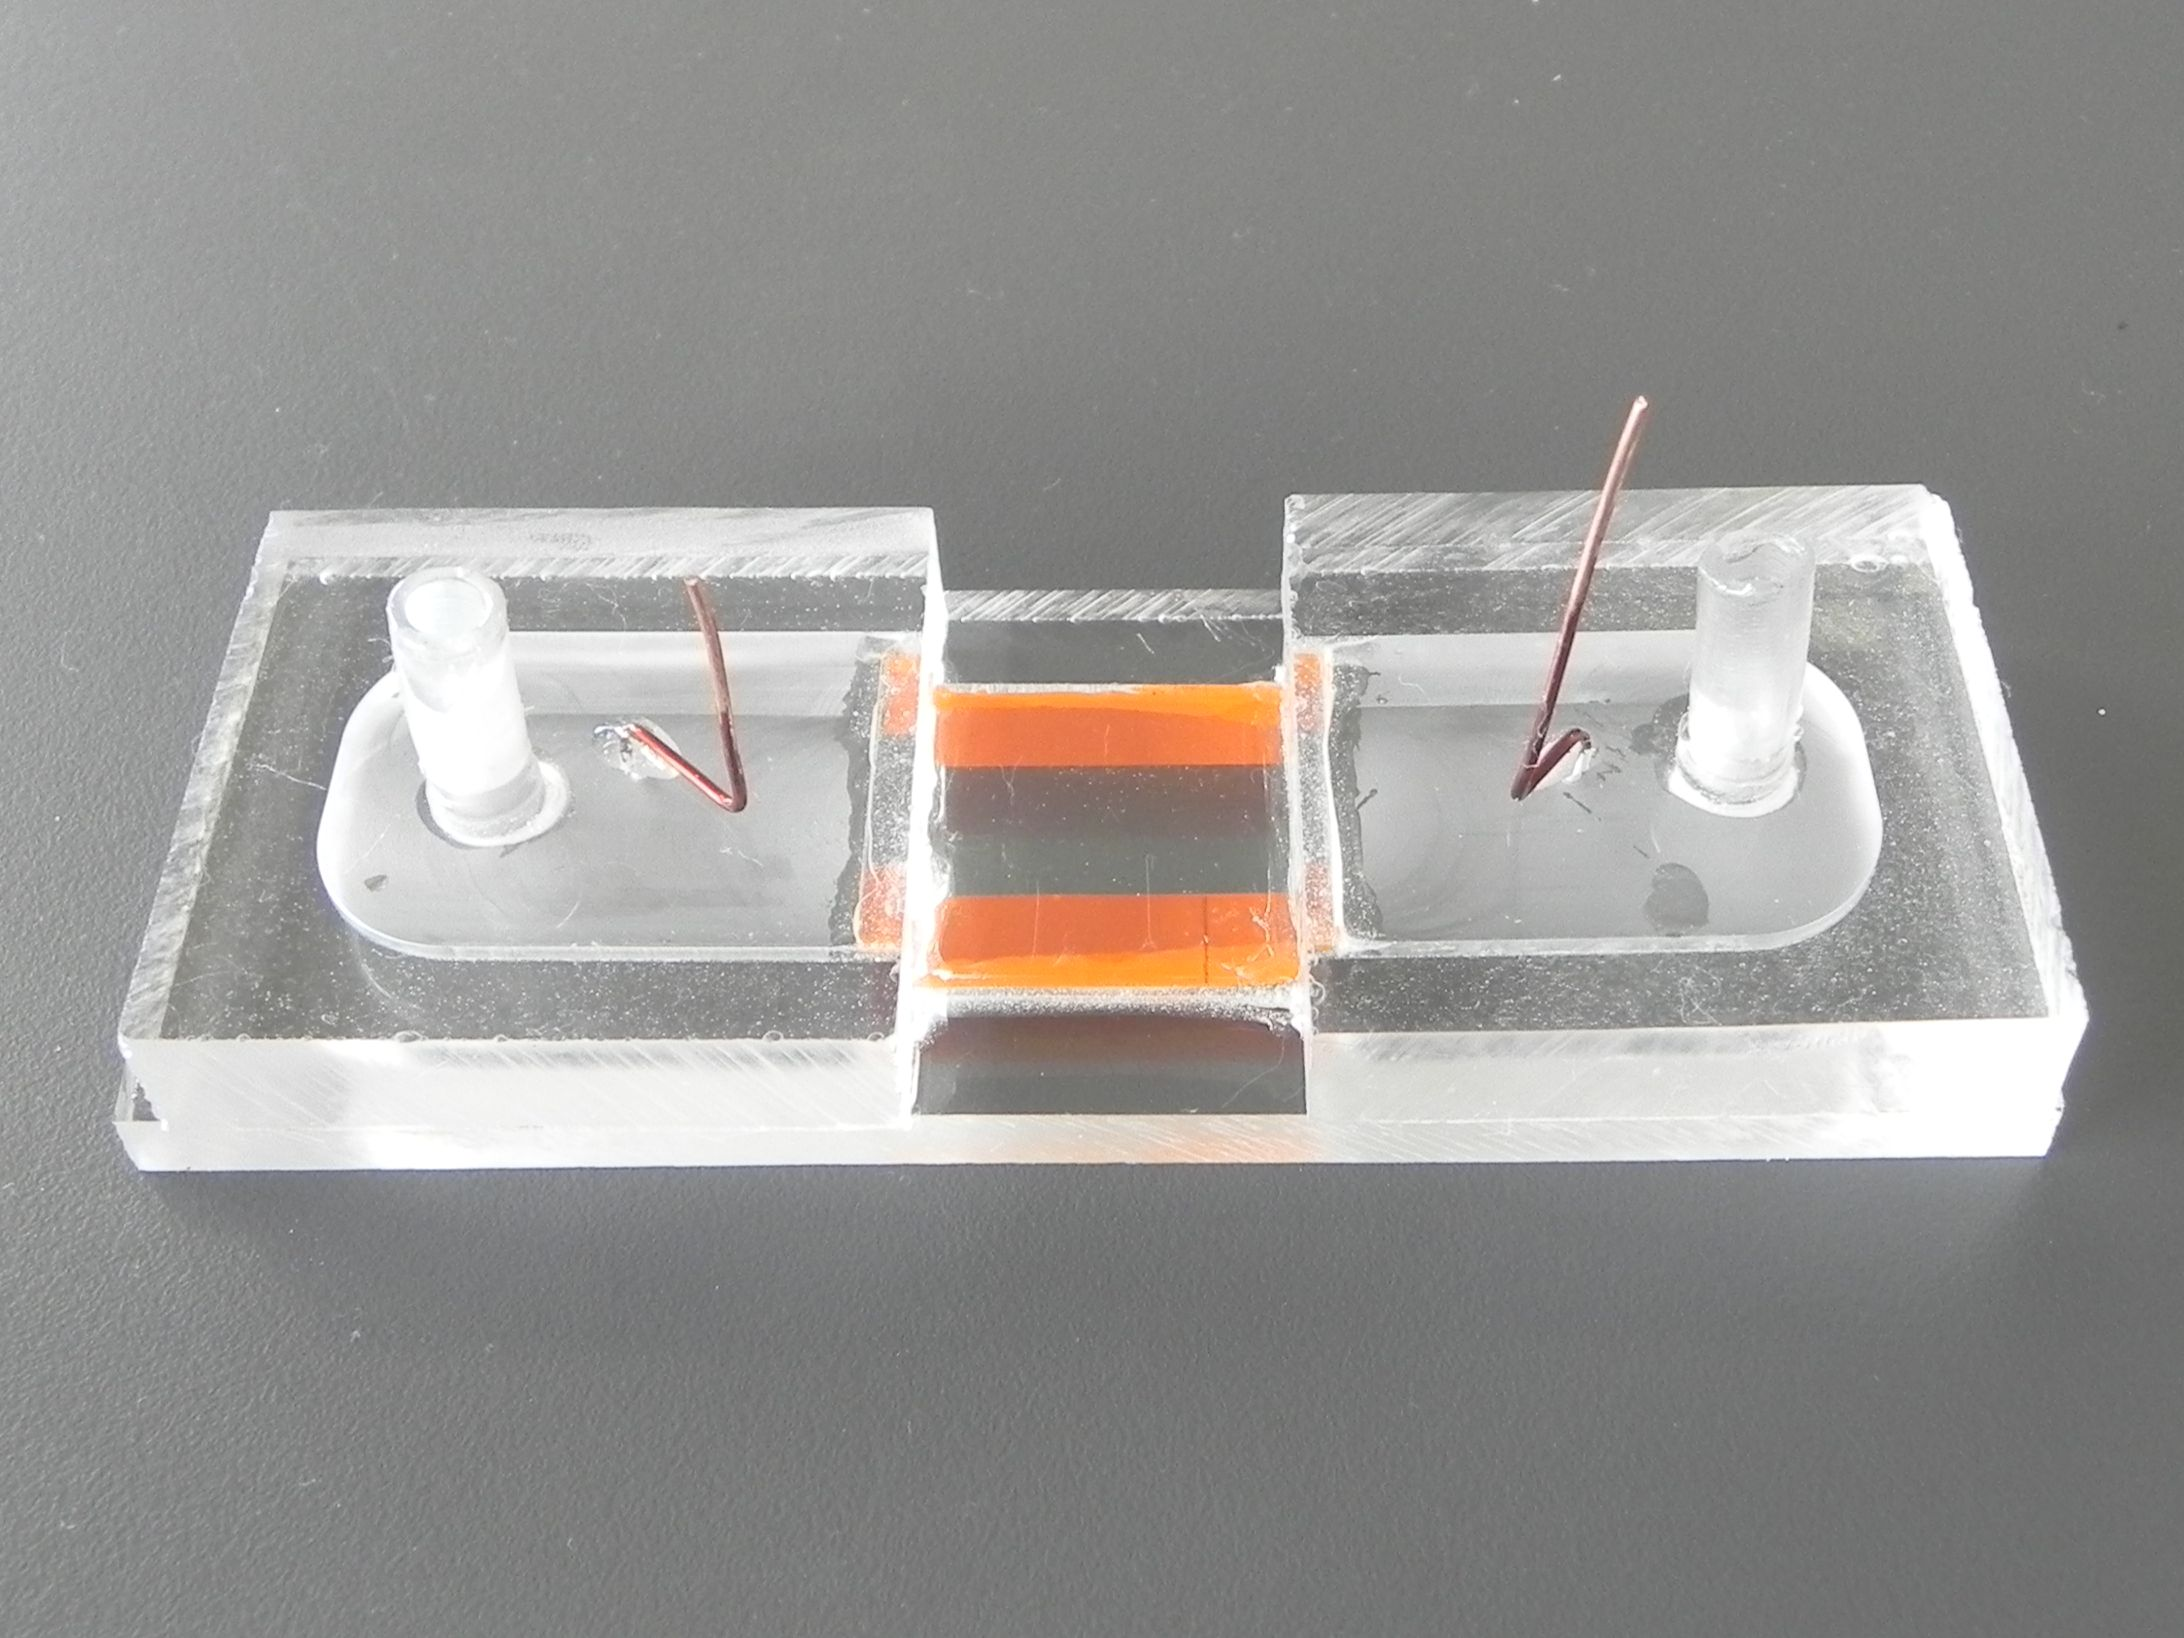
\includegraphics[width=0.5\textwidth]{content/pt1/01-PowerHarvesting/graphics/Photo_streamingPotential_Assembly_Step3.JPG}
      \caption{\label{fig:Photo_streamingPotential_Assembly_Step3}Photo showing final assembly}
    \end{figure}

    \subsubsection*{Construction}

      Construction begins by sectioning standard microscope slides into halves.
      This gives glass panels of approximately \SI{26}{\milli\meter} $\times$ \SI{38}{\milli\meter} $\times$ \SI{1}{\milli\meter}.
      A single panel is then epoxied to an acrylic base plate, as is shown in Figure~\ref{fig:Photo_streamingPotential_Assembly_Step1}.

      Once set, plastic shims are cut to the required size, covered with a very thin layer of epoxy, and placed along the edges of the slide.
      The shims line the sides of the glass panel such that they leave a \SI{1}{\centi\meter} gap through the centre.
      A second glass slide is then placed on top of the shims and epoxy resin is used to seal the sides.
      Pressure was applied to the stack while the epoxy set to ensure the epoxy was distributed correctly and to control the channel height.
      A photo of the shims glued between the two slide halves is shown in Figure~\ref{fig:Photo_streamingPotential_Assembly_Step2}.

      Once set, each channel is examined under a microscope to determine the internal channel height.
      Each of the four corners were measured to ensure the internal dimensions remained rectangular once set.

      \begin{table}
        \begin{tabular}{r|c|l}
          Item & Brand & Product details\tabularnewline\hline
          Microscope slides & Sail Brand & JIA 7101WT - 26 x 76mm\tabularnewline
          Shims & Garlock & Colorplast - 50$\,\mu$m,80$\,\mu$m, 120$\,\mu$m and 250$\,\mu$m\tabularnewline
          Epoxy & Selleys & Araldite - Ultra Clear Resin\tabularnewline
          Pressure sensor & Honeywell & 24PC15SMT - 0 -- $\pm$15 PSI\tabularnewline
        \end{tabular}
        \caption{\label{Table_StreamingCell_MaterialsUsed}Table of materials used to construct the streaming potential cells}
      \end{table}

      To finish, acrylic reservoirs where mounted over each end of the channel.
      These reservoirs facilitate the connection of fluid tubes and voltage probes to each end of the channel.
      The final assembly is shown in Figure \ref{fig:Photo_streamingPotential_Assembly_Step3}.
      A full list of materials used to construct the channels is presented as Table~\ref{Table_StreamingCell_MaterialsUsed}.

      A total of ten channels were made and tested using this method.


\section{Measurements}

Of the papers describing experiments using streaming potential cells (\cite{Gu2000,Mala1997,Scales1992,VanderHeyden2006}), I chose that of Gu and Li to replicate~\cite{Gu2000}.
This was because, at the time, it was the only paper I was aware of.
Their method employs a simple cell design, discussed in the previous section, and a detailed description of the experimental procedure.
This section details the fabrication and measurement of a number of streaming cells.

\subsection{\label{sub:Experimental-Procedure}Experimental setup}

    Measurement of the harvester's output was made in a laboratory with high-sensitivity measurement apparatus and a lab tap for the application water pressure.
    The cells output power was measured with a precision source measurement unit (SMU) and applied pressure was monitored with a differential pressure sensor.

    The Agilent E5270B is a mainframe system that holds banks of SMUs with connections to a GPIB computer interface.
    The Department of Engineering's E5270 contains three SMUs, each having the ability to measure currents as low as one femto-ampere.
    The device uses separate `force' and `sense' connections to ensure the voltage/current being set is accurately controlled where they meet.
    Additionally, it uses tri-axial cables to minimise any interference from outside sources; important when measuring such low currents.

    The input resistance to the E5270's measurement units are specified as \SI{13}{\giga\ohm}.
    It is essential to use such a high impedance measurement due to the high internal resistance of the cell.
    I later show that the internal electrical resistance of the cell is in the order of \SI{5}{\mega\ohm}, so the E5270's input impedance is roughly two thousand times larger.
    If using a lab multimeter, typical internal resistance of \SI{10}{\mega\ohm}, its internal resistance is too close to that of the cells and will affect the measured output.

    The pressure sensor used was a Honeywell 26PC SMT Series differential pressure sensor.
    It comes as surface mount package, making it a cost effective solution, but delicate to set up.
    On its exterior are two ports to which rubber tubes are attached.
    Between those ports, internal to the sensor, sits a diaphragm.
    That diaphragm controls the resistance between two nodes in the sensor's bridge circuit (shown in figure \ref{fig:PressureSensorSchematic}).
    \begin{figure}
        \centering
        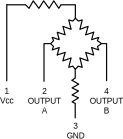
\includegraphics{content/pt1/01-PowerHarvesting/graphics/PressureSensorSchematic}
        \caption{\label{fig:PressureSensorSchematic}Circuit diagram of the differential pressure sensor bridge circuit (taken from \cite{Honeywell2003})}
    \end{figure}
    By applying \SI{10}{\volt} DC between the `Vcc' and `GND' pins, the output voltage between outputs `A' and `B' correspond to the applied pressure.
    Measurement of that output voltage was done using the precision measurement mainframe.

    The mainframe was controlled from a PC running Python scripts utilising the open source Python-vxi11 library~\cite{Python-ivi2014}.
    This allows sweeping the amount of current drawn from the harvester while recording the corresponding voltage drop.
    This is the equivalent of varying the load resistance, which allows us to find the point of maximum power transfer.

    \Cref{fig:measurementSetup} shows the measurement setup as a diagram.
    It shows connection of the measurement mainframe, bench-top power supply, streaming cell, pressure sensor, and the lab tap.
    Table~\ref{tab:measurementSetup_legend} provides details of the abbreviated electrical connection labels used in the figure~\ref{fig:measurementSetup}.

    \begin{figure}
        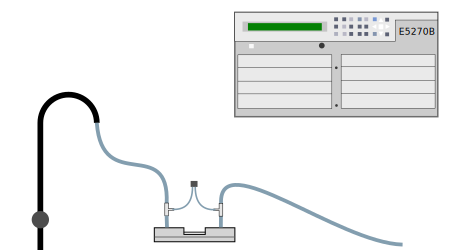
\includegraphics{content/pt1/01-PowerHarvesting/graphics/measurementSetup}
        \caption{\label{fig:measurementSetup}Diagram of equipment setup while measuring power output from the streaming cell harvesters}
    \end{figure}

    \begin{table}
        \centering
        \begin{tabular}{r|l}
        CELL - A & Voltage/current at high-pressure side of cell\\
        PRESS. - A & Output A of pressure sensor\\
        PRESS. - B & Output B of pressure sensor\\
        CELL - B & Voltage/current at low-pressure side of cell
        \end{tabular}
        \caption{\label{tab:measurementSetup_legend}Description of labels used in the streaming cell measurement setup diagram}
    \end{table}

    \subsubsection*{Measurement issues}

    There are two issues with the measurement setup that may impact the measurements.
    Firstly, the electrodes used were copper and are susceptible to polarisation by electrolysis.
    Secondly, the differential pressure sensor is only rated to 15\thinspace PSI (approximately \SI{100}{\kilo\pascal}), less than half the maximum pressure developed across the cell.

    Electrolysis on at the electrode surface causes the electrodes to polarise.
    This results in a semi-permanent offset voltage appearing between the electrodes.
    That offset voltage is opposite in polarity to what is developed while cell is in operation.
    By reversing the flow of water through the cell, the polarisation can be reversed.
    Use of more suitable electrode materials would reduce this effect, for instance platinum black electrodes.
    Copper was used for the electrodes as it was cheap, easily obtainable, and easy to work with.

    From measurement of the output \emph{voltage} of the cells, the presented graphs and figures have been adjusted to remove the effects of electrolysis.
    This was done by adding an offset to the measured data to shift the y-intercept up to \SI{0}{\volt}.
    This provides a more accurate representation of the situation had platinum black electrodes been used.
    As no absolute data is taken from these measurements, the y-intercept adjustment does not affect any subsequent predictions made about the cells.
    Only the gradient of the output, relative to the pressure applied is used; and even then, only to select a suitable candidate cell for power measurement.
    \emph{Most importantly}, no offsets have been applied to measurements of the cell power output.

    Although the maximum rated pressure of sensor was 15\thinspace PSI (approximately \SI{100}{\kilo\pascal}), the sensor's output remained linear up to our maximum pressure of 40\thinspace PSI (\SI{275}{\kilo\pascal}).
    I expect that exceeding the sensors specified pressure will result in a lower `mean time to failure', but its output remained true.
    As a precaution, a tyre pressure gauge was used to roughly confirm the output of the sensor at the end of the cell measurements.
    This was a crude test, however it's output matched that of the differential pressure sensor, so was taken as a good indication of its accuracy.

\subsection{Results}

Results from streaming cell measurement are broken into two sub-sections.
The first presents the output voltage of the ten cells in response to applied water pressure.
From these measurements, the cell with the highest voltage/pressure ratio is found.
The second sub-section shows the maximum power that can be harvested from that cell.
These are the most important measurements as they reveal the energy conversion efficiency of the cells.

\subsubsection*{Voltage versus pressure:}


\begin{figure}[p]
    \centering
    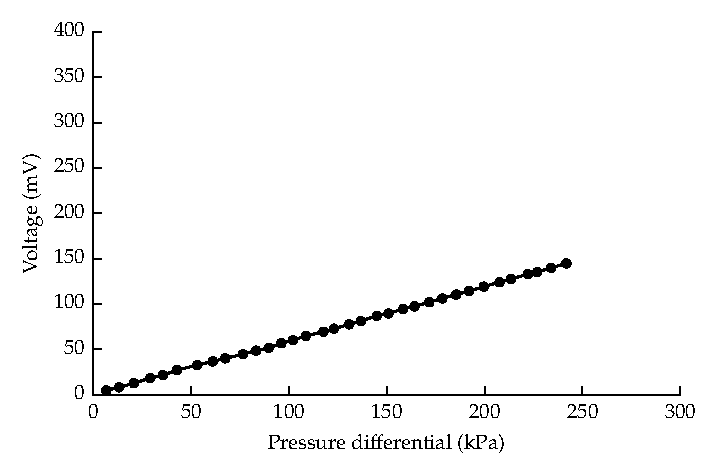
\includegraphics{content/pt1/01-PowerHarvesting/graphics/streamingCell_voltVsPress_26um_out}
    \caption{\label{fig:VvsP_26um}Graph showing the voltage output with applied pressure differential across a \SI{26}{\micro\metre} glass micro-channel (\SI{38}{\milli\volt} offset added)}
\end{figure}

\begin{figure}
    \centering
    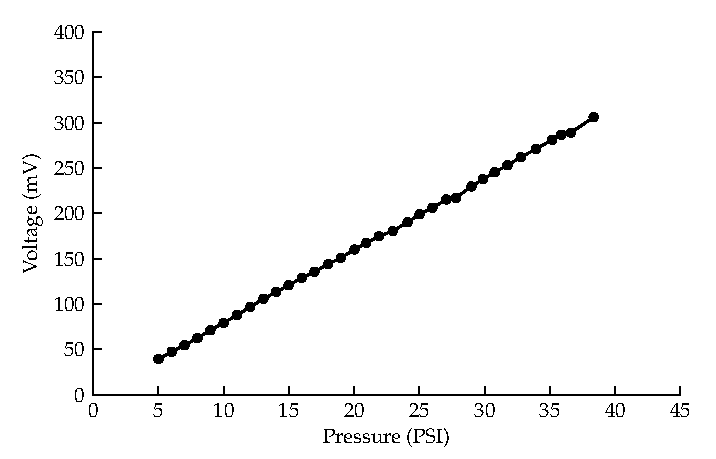
\includegraphics{content/pt1/01-PowerHarvesting/graphics/streamingCell_voltVsPress_52um_out}
    \caption{\label{fig:VvsP_52um}Graph showing the voltage output with applied pressure differential across a \SI{52}{\micro\metre} glass micro-channel (\SI{23}{\milli\volt} offset added)}
\end{figure}

\begin{figure}
    \centering
    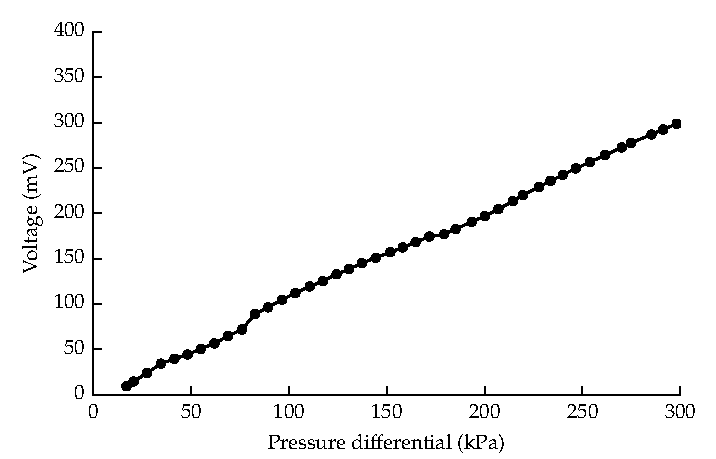
\includegraphics{content/pt1/01-PowerHarvesting/graphics/streamingCell_voltVsPress_56um_out}
    \caption{\label{fig:VvsP_56um}Graph showing the voltage output with applied pressure differential across a \SI{56}{\micro\metre} glass micro-channel (\SI{405}{\milli\volt} offset added)}
\end{figure}

\begin{figure}
    \centering
    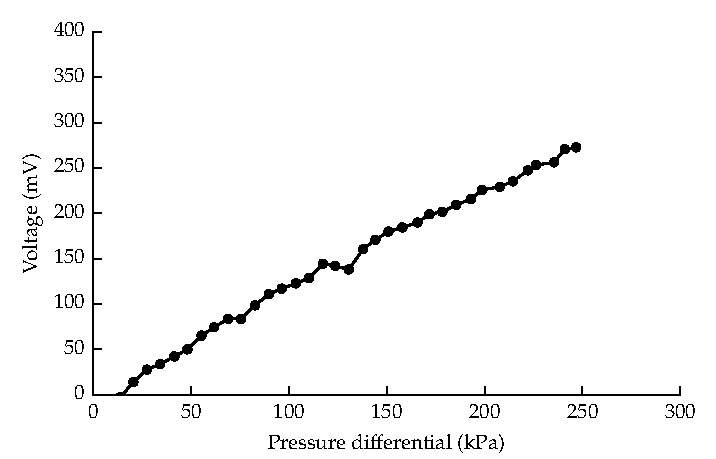
\includegraphics{content/pt1/01-PowerHarvesting/graphics/streamingCell_voltVsPress_71um_out}
    \caption{\label{fig:VvsP_71um}Graph showing the voltage output with applied pressure differential across a \SI{71}{\micro\metre} glass micro-channel (\SI{44}{\milli\volt} offset added)}
\end{figure}

\begin{figure}
    \centering
    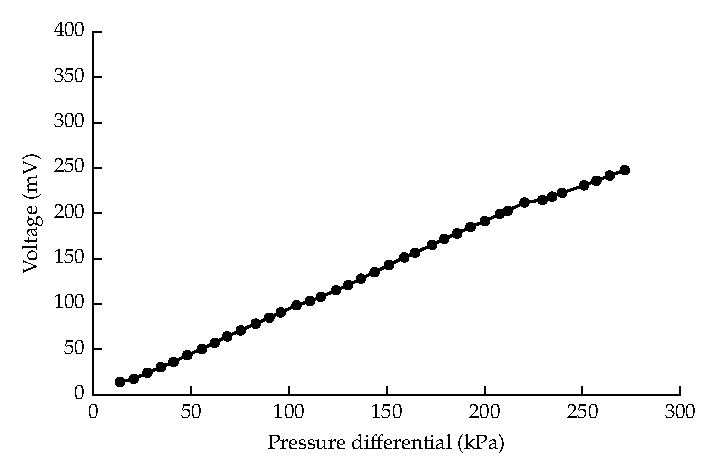
\includegraphics{content/pt1/01-PowerHarvesting/graphics/streamingCell_voltVsPress_75um_out}
    \caption{\label{fig:VvsP_75um}Graph showing the voltage output with applied pressure differential across a \SI{75}{\micro\metre} glass micro-channel (\SI{20}{\milli\volt} offset added)}
\end{figure}

\begin{figure}
    \centering
    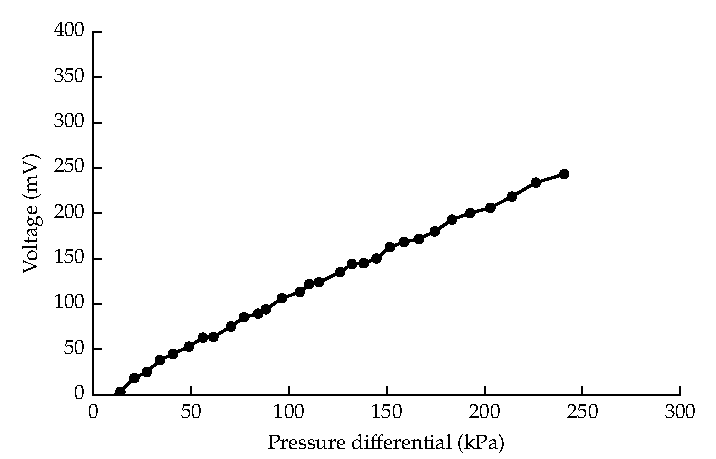
\includegraphics{content/pt1/01-PowerHarvesting/graphics/streamingCell_voltVsPress_106um_out}
    \caption{\label{fig:VvsP_106um}Graph showing the voltage output with applied pressure differential across a \SI{106}{\micro\metre} glass micro-channel (\SI{56}{\milli\volt} offset added)}
\end{figure}

\begin{figure}
    \centering
    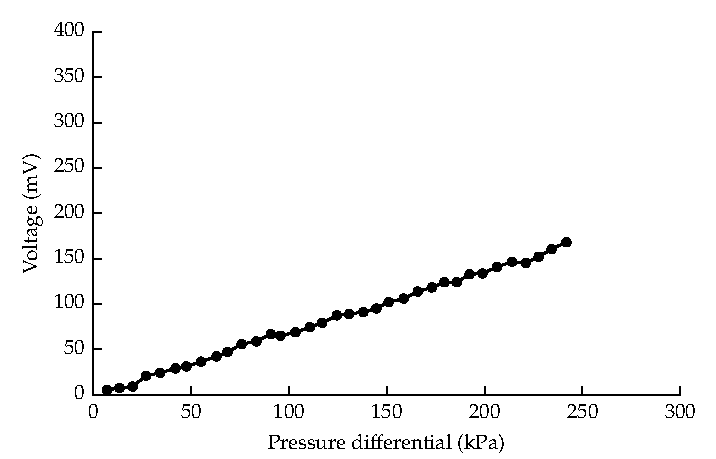
\includegraphics{content/pt1/01-PowerHarvesting/graphics/streamingCell_voltVsPress_125um_out}
    \caption{\label{fig:VvsP_125um}Graph showing the voltage output with applied pressure differential across a \SI{125}{\micro\metre} glass micro-channel (\SI{5}{\milli\volt} offset added)}
\end{figure}

\begin{figure}
    \centering
    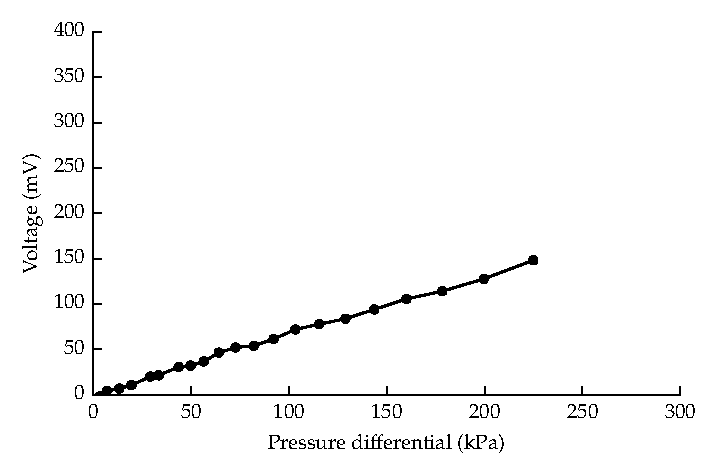
\includegraphics{content/pt1/01-PowerHarvesting/graphics/streamingCell_voltVsPress_161um_out}
    \caption{\label{fig:VvsP_161um}Graph showing the voltage output with applied pressure differential across a \SI{161}{\micro\metre} glass micro-channel (\SI{23}{\milli\volt} offset added)}
\end{figure}

\begin{figure}
    \centering
    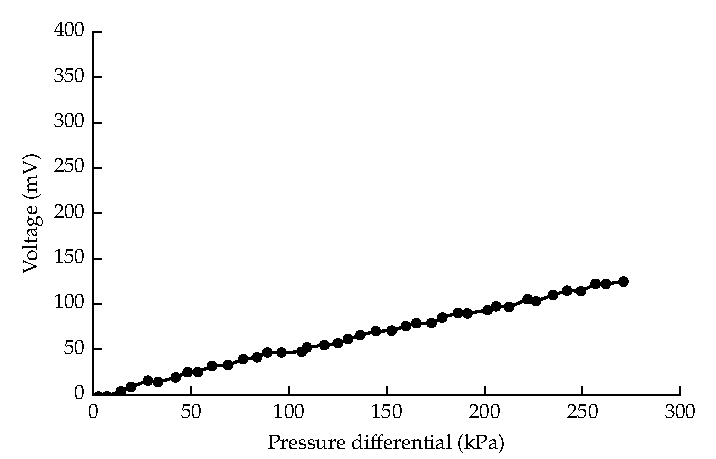
\includegraphics{content/pt1/01-PowerHarvesting/graphics/streamingCell_voltVsPress_178um_out}
    \caption{\label{fig:VvsP_178um}Graph showing the voltage output with applied pressure differential across a \SI{178}{\micro\metre} glass micro-channel (\SI{13}{\milli\volt} offset added)}
\end{figure}

\begin{figure}
    \centering
    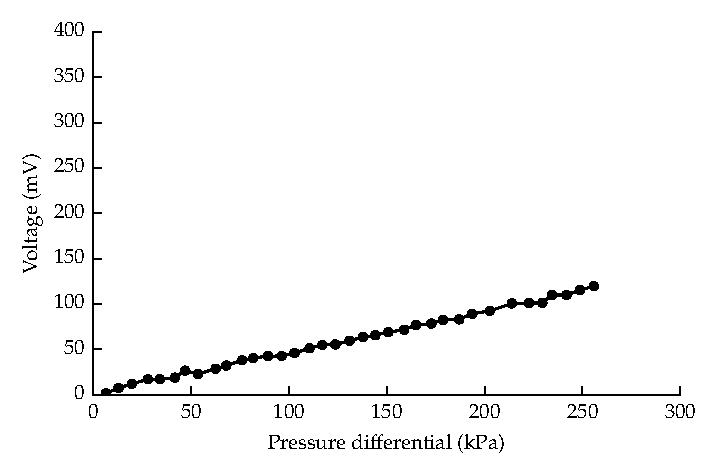
\includegraphics{content/pt1/01-PowerHarvesting/graphics/streamingCell_voltVsPress_245um_out}
    \caption{\label{fig:VvsP_245um}Graph showing the voltage output with applied pressure differential across a \SI{245}{\micro\metre} glass micro-channel (\SI{27}{\milli\volt} offset added)}
\end{figure}

\Crefrange{fig:VvsP_26um}{fig:VvsP_245um} show adjusted results of streaming voltage measurements from each of the ten cells.
They represent the first successful measurements I had made of streaming cells.
During these measurements three cells burst under pressure; two were dropped and subsequently shattered; and one suffered epoxy failure, loosing its acrylic base plate.

No measurements of flow rate or output current were made during these early experiments.
As a result they reveal very little about the efficiency of the cells themselves.
We cannot determine either the mechanical energy put into the cells, nor the output power available.
However, we can relate these measurements to those made by Gu and Li; as will be shown and discussed shortly.

\begin{figure}
    \centering
    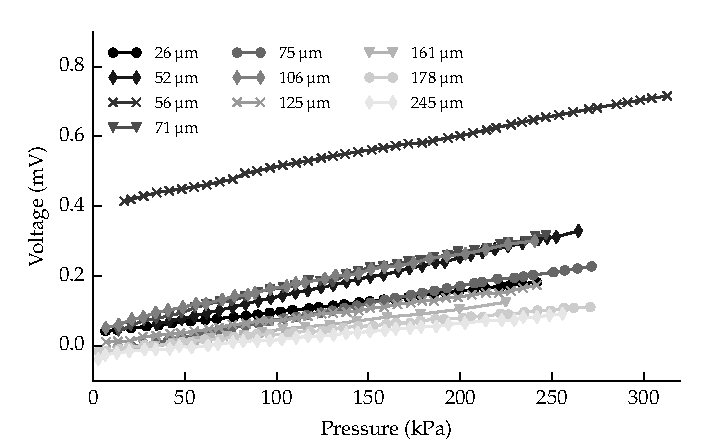
\includegraphics{content/pt1/01-PowerHarvesting/graphics/graph_streamingVoltageGradient_vs_height_noCorrection}
    \caption{\label{fig:streamingCell_all_unadjusted}Plot showing un-adjusted streaming voltages versus applied pressure.}
\end{figure}

\begin{figure}
    \centering
    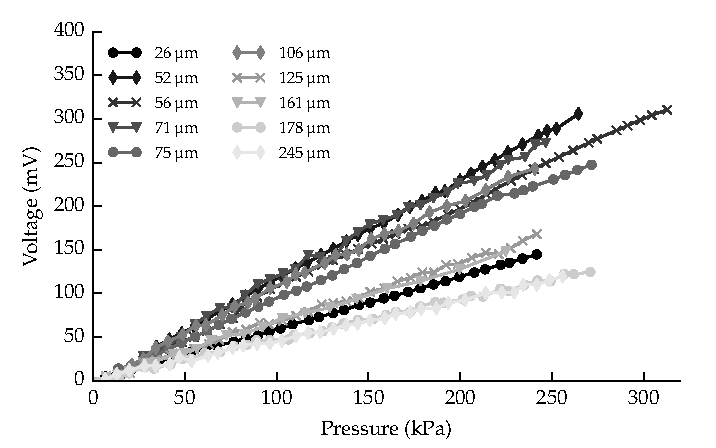
\includegraphics{content/pt1/01-PowerHarvesting/graphics/graph_streamingVoltageGradient_vs_height}
    \caption{\label{fig:streamingCell_all_adjusted}Plot showing adjusted streaming voltages versus applied pressure.}
\end{figure}

\begin{figure}
    \centering
    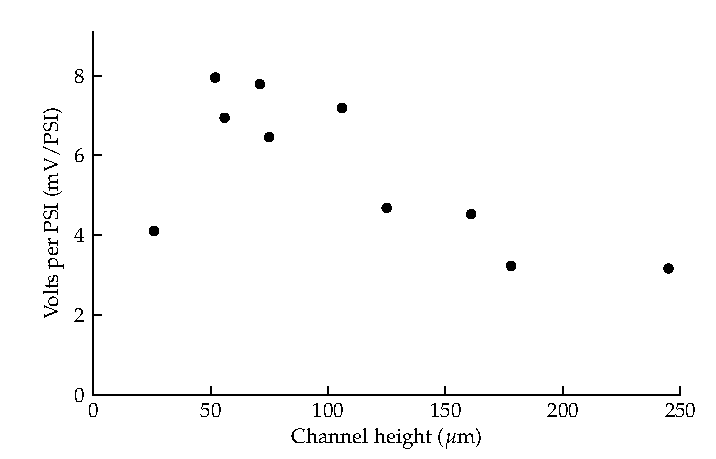
\includegraphics{content/pt1/01-PowerHarvesting/graphics/streamingCell_slopeVsChannelHeight}
    \caption{\label{fig:streamingCell_scatter_voltGradVsHeight}Scatter plot of voltage/pressure gradient versus channel height for each of the measured channels.}
\end{figure}

\Cref{fig:VvsP_56um} required an offset adjustment of \SI{405}{\milli\volt} before its slope gave a \SI{0}{\milli\volt} intercept.
This indicates that the electrodes were highly polarised by the time the measurements were made.
This effect is especially evident in \cref{fig:streamingCell_all_unadjusted}, where each of the traces have been placed on a single graph.

Some of the traces exhibit a certain amount of `jitter' in their pressure-to-voltage gradients.
This is likely due to the time difference between adjacent measurement points.
Measurement points were not taken monotonically, instead being extracted from a number of pressure cycles.

The effect of adding the offset adjustments is visible in \cref{fig:streamingCell_all_adjusted}.
These adjustments bring all of the slopes together so the origin sits at \SI{0}{\volt\per\pascal}.

\Cref{fig:streamingCell_scatter_voltGradVsHeight} shows the streaming voltage to pressure gradients versus channel height.
This data has been taken from the previous graph (\cref{fig:streamingCell_all_adjusted})) to show the response as a function of channel height.

\subsubsection*{Power versus output resistance}

\begin{figure}
    \centering
    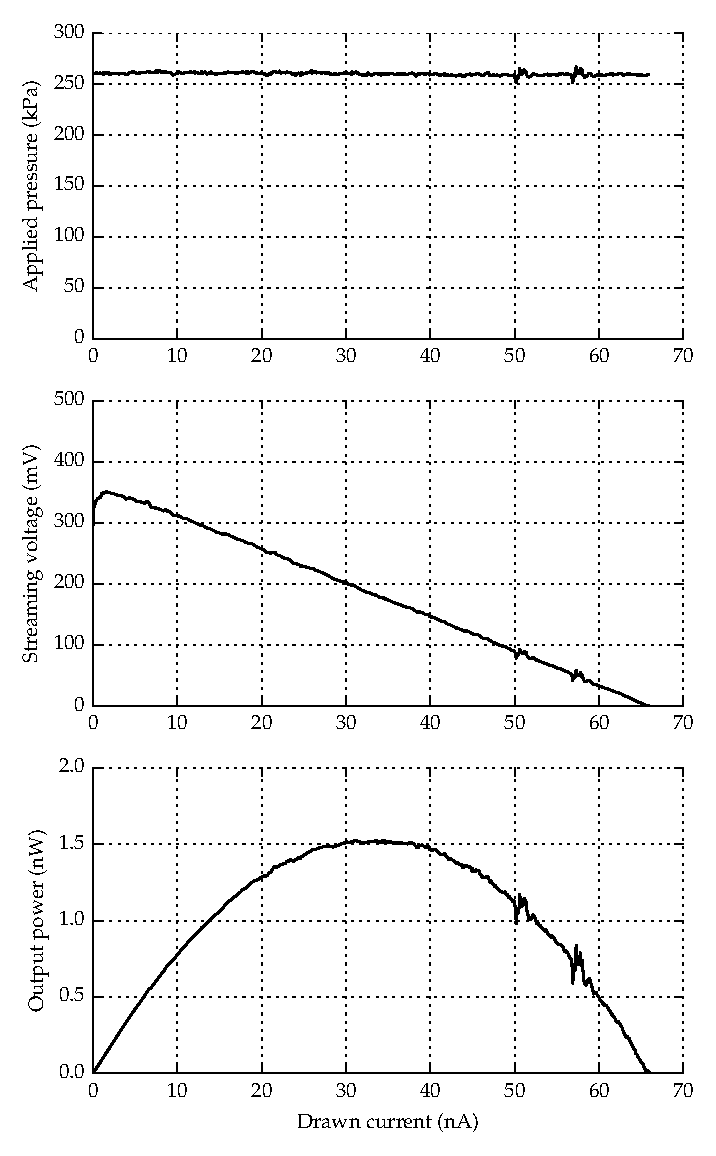
\includegraphics{content/pt1/01-PowerHarvesting/graphics/graph_streamingCell_outputPower_resistanceSweep}
    \caption{\label{fig:streamingCell_maxPower}Plot of output power versus effective load resistance for a \SI{71}{\micro\metre} high channel at a pressure of \SI{260}{\kilo\pascal}.}
\end{figure}

\Cref{fig:streamingCell_maxPower} shows the characteristic power curve of a the \SI{71}{\micro\meter} high streaming cell channel.
Pressure fluctuations near the end of the experiment are due to usage of the departments water system.
Their effect is visible in both the streaming voltage and output power traces, highlighting the strong coupling to applied pressure.

The maximum power delivered by the cell was \SI{1.52}{\nano\watt}, corresponding to a current draw of \SI{33.5}{\nano\ampere} with a streaming voltage of \SI{182}{\milli\volt}.
Generating this power required \SI{260}{\kilo\pascal} of pressure, resulting in a flow rate of \SI{2.05}{\milli\litre\per\second}.
This equates to \SI{539}{\milli\watt} of pumping power lost to the device and therefore an energy conversion efficiency of \SI{0.28}{\micro\percent}.

\subsection{Discussion}

Initial measurements of streaming voltage revealed that the output voltage is directly proportional to applied pressure.
Containing pressures reaching \SI{260}{\kilo\pascal} within glass structures is difficult.

Comparing the streaming voltage measurements taken from each of the ten cells to the measurements make by Gu and Li yielded surprising results.
In their paper~\cite{Gu2000}, they determined the zeta potential ($\zeta$) and surface conductivity ($\lambda$) by plotting measurements and fitting a linear equation to their data.
The use the y-intercept of the resulting line to give the inverse zeta potential and the slope of the line gave information about the surface conductivity.

\begin{figure}
    \centering
    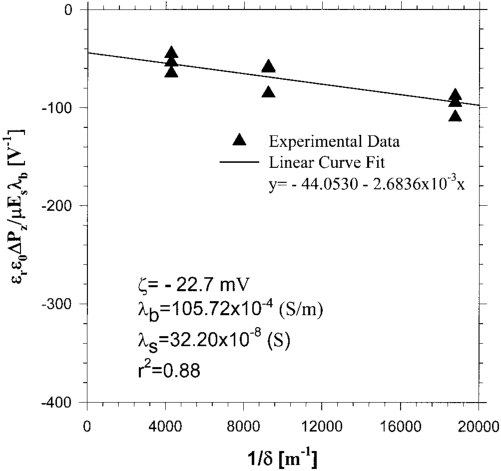
\includegraphics{content/pt1/01-PowerHarvesting/graphics/GuLi_DIUF}
    \caption{\label{fig:Gu_Li_comparison_DUIF}Measured data from Gu and Li's paper on streaming cells relating the streaming voltage and pressure differential to the channel height with distilled water as the working fluid}
\end{figure}

\begin{figure}
    \centering
    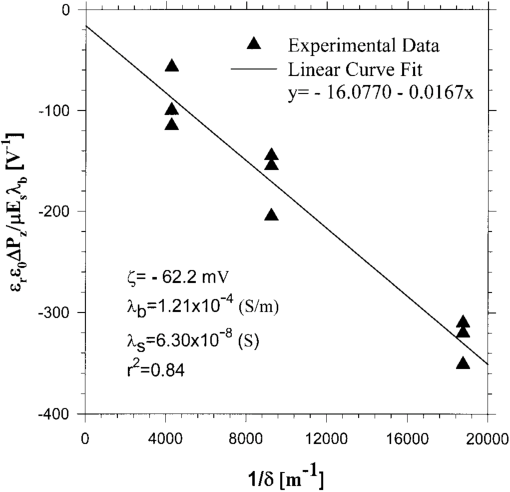
\includegraphics{content/pt1/01-PowerHarvesting/graphics/GuLi_NaCl}
    \caption{\label{fig:Gu_Li_comparison_NaCl}Measured data from Gu and Li's paper on streaming cells relating the streaming voltage and pressure differential to the channel height with a \SI{1}{\milli\mole} sodium chloride solution as the working fluid}
\end{figure}

Their results for three streaming cells are shown here (taken from \cite{Gu2000}) as \cref{fig:Gu_Li_comparison_DUIF,fig:Gu_Li_comparison_NaCl}.
The first (\cref{fig:Gu_Li_comparison_DUIF}) shows measurements when distilled water is used as the working fluid; the second (\cref{fig:Gu_Li_comparison_NaCl}) shows the measurements for a weak saline solution.
It is interesting to note that they have what looks to be fairly linear data, although it is hard to tell with only three channel sizes.

\begin{figure}
    \centering
    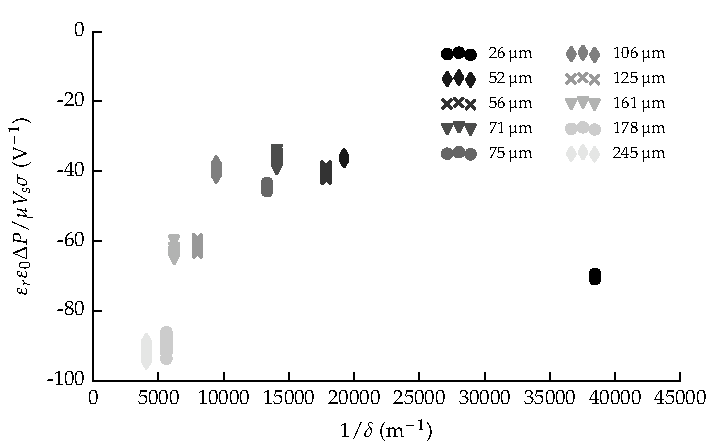
\includegraphics{content/pt1/01-PowerHarvesting/graphics/graph_streamingComparison_gu}
    \caption{\label{fig:streamingCell_scatter_Gu_Li}Scatter plot with results of streaming cell measurements in terms of those made by Gu and Li~\cite{Gu2000} (for comparison).}
\end{figure}

By comparison, \cref{fig:streamingCell_scatter_Gu_Li} plots the same variables from measurements taken from the ten streaming cells fabricated here.
In this graph $\lambda{b}$ has been replaced with $\sigma$, where both refer to the bulk conductivity of the solution; and $E_{s}$ has been replaced with $V_{s}$, were both refer to the streaming potential.
The response to variation of channel height is clearly non-linear.
Their method of finding the zeta potential rests on the following rearrangement:
\begin{eqnarray}
    \frac{\varepsilon_{r}\varepsilon_{0}\Delta P}{\mu V_{s}\sigma} = \frac{1}{\zeta} + \left( \frac{2\,\lambda}{\zeta \sigma}\right)\,\frac{1}{\delta}
\end{eqnarray}
where $\lambda$ is the surface conductivity and $\delta$ is the channel height.
So as the channel height ($\delta$) tends to infinity, the left hand side tends toward the zeta potential ($\zeta$).
This notion seems counter intuitive since the zeta potential is defined at the plane of sheer (as shown in \cref{fig:doubleLayer_anatomy}), relative to the solution bulk.
The equation is stating that no-matter how far you separate the walls, the minimum voltage-pressure gradient you can get is still set by the zeta potential.

Measurement of the output power generated by the \SI{71}{\micro\meter} streaming cell are promising.
From this measurement the power transfer curve is evident.
Referring back to the model presented as \cref{fig:StreamingCell_Schematic-representation}, we can now calculate the channels internal electrical resistance ($R_{cell}$).
We know from the graph that the maximum power transfer occurred at a current of \SI{33.5}{\nano\ampere} with a streaming voltage of \SI{182}{\milli\volt}.
Via Ohm's law this equates to a load resistance ($R_{out}$) of \SI{5.43}{\mega\ohm}, which from the maximum power theorem we know must be equal to the cells internal resistance.




% If we remove the constants and isolate the case where we end up with just the zeta potential we get:
% \begin{eqnarray}
%     \frac{\varepsilon_{r}\varepsilon_{0}\Delta P}{\mu V_{s}\sigma} &=& \frac{1}{\zeta} + \left( \frac{2\,\lambda}{\zeta \sigma}\right)\,\frac{1}{\delta}\nonumber\\
%     \frac{\varepsilon_{r}\varepsilon_{0}\Delta P}{\mu V_{s}\sigma} &=& \frac{1}{\zeta} + \frac{2\lambda}{\zeta\delta\sigma}\nonumber\\
%     \frac{\varepsilon_{r}\varepsilon_{0}\Delta P}{\mu V_{s}\sigma} &=& \frac{\zeta\delta\sigma + 2\zeta\lambda}{\zeta^{2}\delta\sigma}\nonumber\\
%     \frac{\varepsilon_{r}\varepsilon_{0}\Delta P}{\mu V_{s}\sigma} &=& \left(\frac{\zeta}{\zeta}\right) \, \frac{\delta\sigma + 2\lambda}{\zeta \delta\sigma}\nonumber\\
%     \frac{\mu V_{s}\sigma}{\varepsilon_{r}\varepsilon_{0}\Delta P} &=& \frac{\zeta \delta\sigma}{\delta\sigma + 2\lambda}\nonumber\\
%     \frac{\mu V_{s}\sigma}{\varepsilon_{r}\varepsilon_{0}\Delta P} &=& \left(\frac{\delta}{\delta}\right) \, \frac{\zeta\sigma}{\sigma + \frac{2\lambda}{\delta}}\nonumber\\
%     \frac{\mu V_{s}\sigma}{\varepsilon_{r}\varepsilon_{0}\Delta P} &=& \frac{\zeta\sigma}{\sigma + \frac{2\lambda}{\delta}}\nonumber\\
%     \frac{\mu V_{s}}{\varepsilon_{r}\varepsilon_{0}\Delta P} &=& \frac{\zeta}{\sigma + \frac{2\lambda}{\delta}}
% \end{eqnarray}


% \begin{eqnarray}
%     \frac{\varepsilon_{r}\varepsilon_{0}\Delta P}{\mu V_{s}\sigma} &=& \frac{1}{\zeta} + \left( \frac{2\,\lambda}{\zeta \sigma}\right)\,\frac{1}{\delta}\nonumber\\
%     \frac{\Delta P}{V_{s}} &\propto& \frac{1}{\zeta} + \left(\frac{\lambda}{\zeta }\right)\,\frac{1}{\delta}\nonumber\\
%     \frac{\Delta P}{V_{s}} &\propto& \frac{1}{\zeta} + \frac{\lambda}{\zeta\delta}\nonumber\\
%     \frac{\Delta P}{V_{s}} &\propto& \frac{\zeta\delta + \zeta\lamda}{\zeta^{2}\delta}\nonumber\\
%     \frac{\Delta P}{V_{s}} &\propto& \left(\frac{\zeta}{\zeta}\right) \, \frac{\delta + \lambda}{\zeta \delta}\nonumber\\
%     \frac{V_{s}}{\Delta P} &\propto& \frac{\zeta \delta}{\delta + \lambda}\nonumber\\
%     \frac{V_{s}}{\Delta P} &\propto& \left(\frac{\delta}{\delta}\right) \, \frac{\zeta}{1 + \frac{\lambda}{\delta}}\nonumber\\
%     \frac{V_{s}}{\Delta P} &\propto& \frac{\zeta}{1 + \frac{\lambda}{\delta}}
% \end{eqnarray}

% The first shows voltage measurements of the ten cells, adjusted to remove the effects of electrolysis.
% From these measurements, the

% Ten cavities ranging in height from 26$\,\mu m$ to 245$\,\mu m$ where built and
% measured. Individual plots showing pressure applied versus voltage developed
% are shown in Appendix \ref{sec:Appendix-Streaming-Potential-Cell}.  For
% convenience, a graph with the steepest voltage per pressure gradient is shown
% in Figure \ref{fig:streamingCell_voltVsPress_52um_convienient}, which resulted
% from using a cell with a height of 52$\,\mu m$.



% From the results obtained it is clear that there is a definite \nobreakdash-
% linear \nobreakdash- relationship between the amount of pressure applied and
% the voltage developed across each channel. Figure
% \ref{fig:streamingCell_scatter_voltGradVsHeight} compares the gradient of
% voltage developed per PSI of pressure for each of the channels. The graph shows
% a trend toward larger voltage development as channel height is reduced to
% around 50$\,\mu m$. Below 50$\,\mu m$ it is unclear what to expect from the
% channel which will require further investigation. Spread in the data is
% expected to be the result of epoxy (used to glue the slides together) seeping
% into the cavity, thereby slightly altering each cavity's dimensions.




\subsection{Conclusion}
Conversion of mechanical pumping into electrical energy can be done with narrowly separated plates of glass.
The conversion efficiency seen here was low, much lower than reported in the literature.
A channel \SI{1}{\centi\meter} by \SI{3}{\centi\meter} by \SI{71}{\micro\meter} produced \SI{1.5}{\nano\watt} under a pressure differential of \SI{260}{\kilo\pascal}.
That took \SI{359}{\milli\watt} of pumping power to produce, yielding an efficiency in the order of \SI{0.1}{\micro\percent}.
Precision engineering, with regards to cell construction, will likely lead to greater efficiency.
This is based on reports from the literature, where higher efficiency channels utilised much narrower channels.

Measurements of ten streaming cells were compared to the results published by Gu and Li.
The linear relationship of Gu and Li between channel height and their plotted parameter could not be reproduced.
Instead, results showed a highly non-linear relationship as shown in~\cref{fig:streamingCell_scatter_Gu_Li}.
The gradient of measurement points within the range of channel heights measured by Gu and Li is reversed.
The reason for the discrepancy is not clear.

Streaming voltage is linear with the applied pressure.
This could potentially be useful as a means of sensing water flow rates.
A dual purpose such as power sourcing and flow measurement lends itself well to water metering applications.
